% Copyright 2025 Fausto Spoto
%
% Licensed under the Apache License, Version 2.0 (the "License");
% you may not use this file except in compliance with the License.
% You may obtain a copy of the License at
%
%    http://www.apache.org/licenses/LICENSE-2.0
%
% Unless required by applicable law or agreed to in writing, software
% distributed under the License is distributed on an "AS IS" BASIS,
% WITHOUT WARRANTIES OR CONDITIONS OF ANY KIND, either express or implied.
% See the License for the specific language governing permissions and
% limitations under the License.

%\RequirePackage{luatex85}
\documentclass[11pt]{beamer}  %% versione proiettore
%%\documentclass[11pt,handout]{beamer} %% versione stampa
\usepackage{lucidiJb-2ed}

\usepackage{animate}
\usepackage{mathtools}
\usepackage{relsize}
\usepackage[normalem]{ulem}
\usepackage[dvipsnames]{xcolor}
\usepackage{amsmath}
\usepackage{amssymb}
\usepackage{amsfonts}
\usepackage{tikz}
%\usetikzlibrary {arrows.meta,graphs,graphdrawing}
%\usegdlibrary{layered}
%\usegdlibrary{trees}
\usetikzlibrary{decorations.pathreplacing}
\usetikzlibrary {arrows.meta}
\usepackage{algorithm,algpseudocode}
\usepackage{listings}

\lstset{
  breakatwhitespace,
  language=MATLAB,
  columns=fullflexible,
  keepspaces,
  breaklines,
  tabsize=3, 
  showstringspaces=false,
  extendedchars=true,
  basicstyle=\fontfamily{pcr}\selectfont\scriptsize,
  keywordstyle=\color{orange},
  upquote=true,
  literate={-}{-}1}

\renewcommand{\algorithmicrequire}{\textbf{Input:}}
\renewcommand{\algorithmicensure}{\textbf{Output:}}

\mode<article>
{
  \usepackage{fullpage}
  \usepackage{hyperref}
}

\mode<presentation>
{
  \setbeamertemplate{background canvas}[vertical shading][bottom=red!10,top=blue!10]
  \usetheme{Course}
  \usefonttheme[onlysmall]{structurebold}
}

\newcommand{\wrt}{\textit{wrt.\ }}
\newcommand{\ie}{, \textit{ie.}, }

\newcommand{\numberofscoops}{{\#\mathit{scoops}}}
\newcommand{\noncesize}{{\mathit{nonce}_{\mathit{size}}}}
\newcommand{\byte}{{\mathit{byte}}}
\newcommand{\nonce}{{\mathit{nonce}}}
\newcommand{\bestNonce}{{\mathit{best\_nonce}}}
\newcommand{\nonces}{{\mathit{nonces}}}
\newcommand{\scoops}{{\mathit{scoops}}}
\newcommand{\plot}{{\mathit{plot}}}
\newcommand{\scoop}{{\mathit{scoop}}}
\newcommand{\seed}{{\mathit{seed}}}
\newcommand{\previous}{{\mathit{previous}}}
\newcommand{\deadline}{{\mathit{deadline}}}
\newcommand{\generation}{{\mathit{generation}}}
\newcommand{\size}{{\mathit{size}}}
\newcommand{\scoopnumber}{{\mathit{scoopNumber}}}
\newcommand{\data}{{\mathit{data}}}
\newcommand{\challenge}{{\mathit{challenge}}}
\newcommand{\delay}{{\mathit{delay}}}
\newcommand{\mynext}{{\mathit{next}}}
\newcommand{\nextchallenge}{\challenge_\mynext}
\newcommand{\initialchallenge}{{\mathit{initialChallenge}}}
\newcommand{\height}{{\mathit{height}}}
\newcommand{\trunk}{{\mathit{trunk}}}
\renewcommand{\block}{{\mathit{block}}}
\newcommand{\oblivion}{{\mathit{oblivion}}}
\newcommand{\now}{{\mathit{now}}}
\newcommand{\beat}{{\mathit{beat}}}
\newcommand{\weightedbeat}{\mathit{weightedBeat}}
\newcommand{\nextweightedbeat}{\weightedbeat_\mynext}
\newcommand{\power}{{\mathit{power}}}
\newcommand{\hash}{{\mathit{hash}}}
\newcommand{\difficulty}{{\mathit{difficulty}}}
\newcommand{\hashfirstk}{{\mathit{hash\ of\ first\ \kappa\ bytes\ of}}}
\newcommand{\previousblockhash}{{\mathit{previousBlockHash}}}
\newcommand{\waitingtime}{{\mathit{waitingTime}}}
\newcommand{\nextwaitingtime}{\tau_\mynext}
\newcommand{\nextpower}{\power_\mynext}
\newcommand{\nextacceleration}{\alpha_\mynext}
\newcommand{\nextblock}{\block_\mynext}
\newcommand{\genesis}{{\mathit{genesis}}}
\newcommand{\consensus}{{\mathit{consensus}}}
\newcommand{\nattobe}{{\mathit{nat2be}}}
\newcommand{\betonat}{{\mathit{be2nat}}}
\newcommand{\finalhash}{{h_{\mathit{final}}}}
\newcommand{\chainidentifier}{{\mathit{chainIdentifier}}}
\newcommand{\publickeyofpeer}{{\mathit{publicKeyOfPeer}}}
\newcommand{\publickeyofminer}{{\mathit{publicKeyOfMiner}}}

\newcommand{\Prologs}{{\mathsf{Prologs}}}
\newcommand{\Plots}{{\mathsf{Plots}}}
\newcommand{\Challenges}{{\mathsf{Challenges}}}
\newcommand{\Scoops}{{\mathsf{Scoops}}}
\newcommand{\Nonces}{{\mathsf{Nonces}}}
\newcommand{\Trunks}{{\mathsf{Trunks}}}
\newcommand{\Blocks}{{\mathsf{Blocks}}}
\newcommand{\GenesisBlocks}{{\mathsf{GenesisBlocks}}}
\newcommand{\NonGenesisBlocks}{{\mathsf{NonGenesisBlocks}}}
\newcommand{\Deadlines}{{\mathsf{Deadlines}}}

\newcommand{\computer}{
\includegraphics[width=1.3cm]{pictures/computer}}
\newcommand{\leftArrow}{
\includegraphics[width=0.6cm]{pictures/left_arrow}}
\newcommand{\signature}{
\includegraphics[width=0.3cm]{pictures/signature}}

\colorlet{alicecolor}{green!90!black}
\colorlet{bobcolor}{red!90!black}
\colorlet{faustocolor}{yellow!90!black}
      
\subtitle{ReACT'25, S\~ao Luis, Brasil, 23/7/2025}
\title{Ecological Cryptomining, Theoretical Background and Concrete Implementation}
\institute{Universit\`a di Verona, Italy}
\date{23/7/2025}

\setbeamercovered{invisible}

\def\codesize{\smaller}
\def\<#1>{\codeid{#1}}
\newcommand{\codeid}[1]{\ifmmode{\mbox{\codesize\ttfamily{#1}}}\else{\codesize\ttfamily #1}\fi}

\AtBeginSection[]{
  \begin{frame}
  \vfill
  \centering
  \begin{beamercolorbox}[sep=8pt,center,shadow=true,rounded=true]{title}
    \usebeamerfont{title}\insertsectionhead\par%
  \end{beamercolorbox}
  \vfill
  \end{frame}
}

\begin{document}

\begin{frame}
  \titlepage
\end{frame}

\begin{frame}{About myself}
  \begin{itemize}
  \item Associate Professor, Department of Computer Science, University of Verona, Italy
  \item software engineering and verification (1995-today)
  \item smart contracts, consensus, blockchain programming (2018-today)
  \end{itemize}

  \medskip

  \begin{center}
    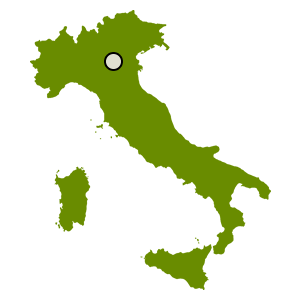
\includegraphics[width=3cm]{pictures/verona_map}
  \end{center}

\end{frame}

\begin{frame}{The IT green dream (1990-2010)}

  \begin{center}
    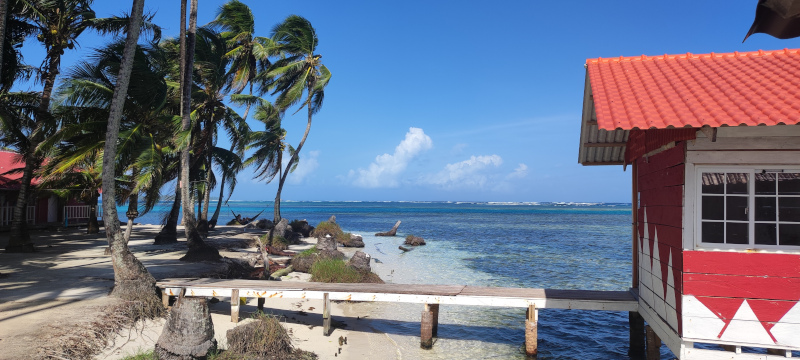
\includegraphics[width=0.7\textwidth]{pictures/green_dream}
  \end{center}

  \begin{center}
    Digital nomads work online from the beach. Calls instead of meetings. No pollution. No war. Peace and love.
  \end{center}

  \begin{center}
    Who needs to think when artificial intelligence things for us?
  \end{center}

  \begin{center}
    Who needs banknotes when we have Bitcoin?
  \end{center}

  \begin{center}
    Who needs a war when we are so social?
  \end{center}

  \begin{center}
    Who needs to drive when cars drive?
  \end{center}

\end{frame}

\begin{frame}{The IT reality ($>$2010)}

  \begin{center}
    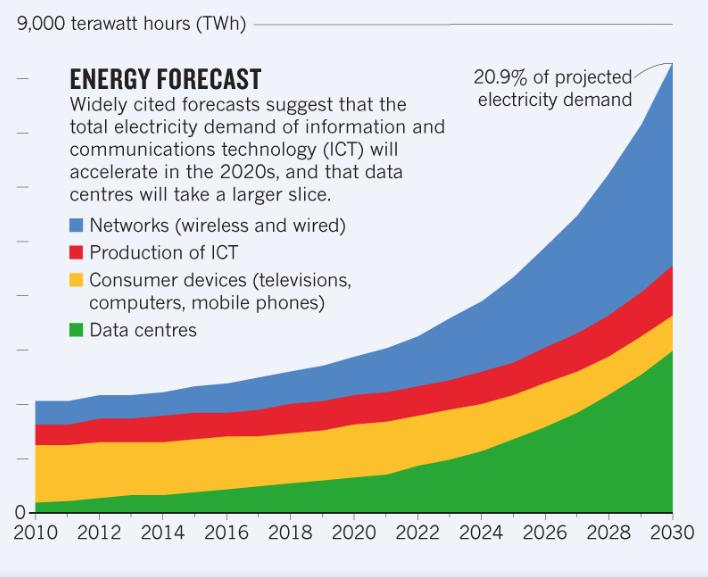
\includegraphics[width=0.7\textwidth]{pictures/forecast}
  \end{center}

  \begin{center}
    {\tiny (source: \url{https://www.capgemini.com/insights/expert-perspectives/the-more-sustainable-data-center/})}
  \end{center}
    
\end{frame}

\begin{frame}{The IT reality ($>$2010)}

  \begin{center}
    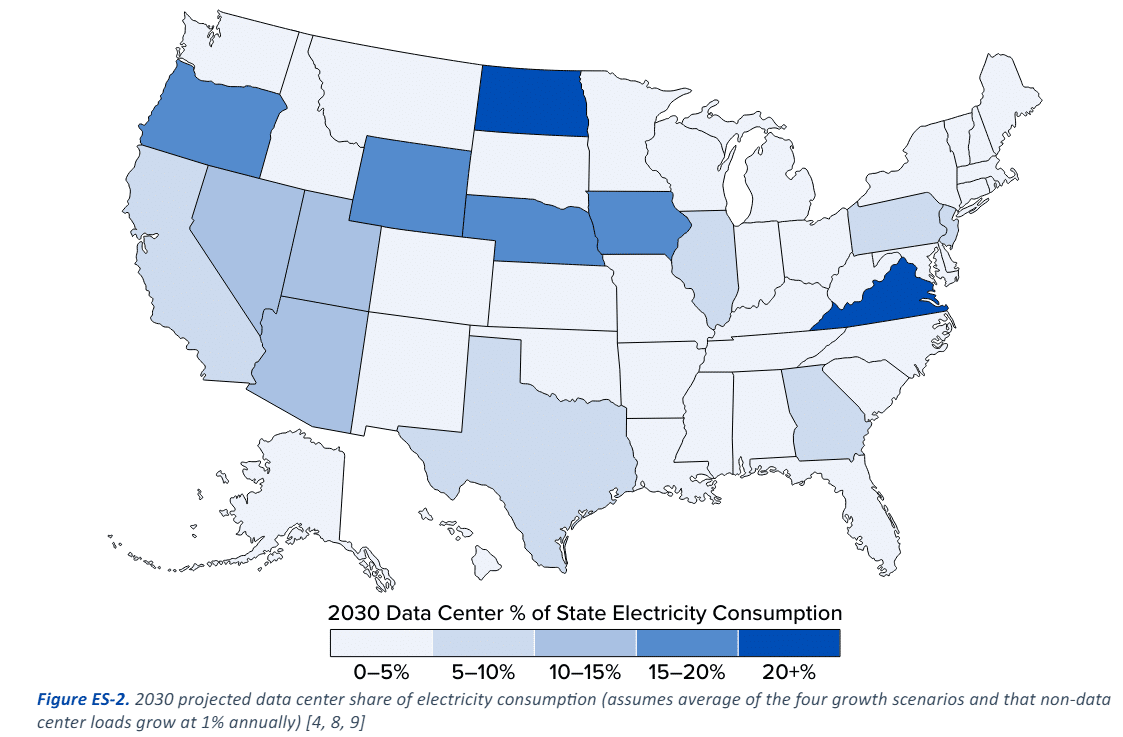
\includegraphics[width=0.7\textwidth]{pictures/data-centers-electricity-use}
  \end{center}

  \begin{center}
    Exercise: find Amazon Web Services in the map
  \end{center}

  \begin{center}
    {\tiny (source: \url{https://carboncredits.com/us-data-centers-power-requirement-will-double-by-2030/})}
  \end{center}

\end{frame}

\begin{frame}{Not just electricity}

  \begin{center}
    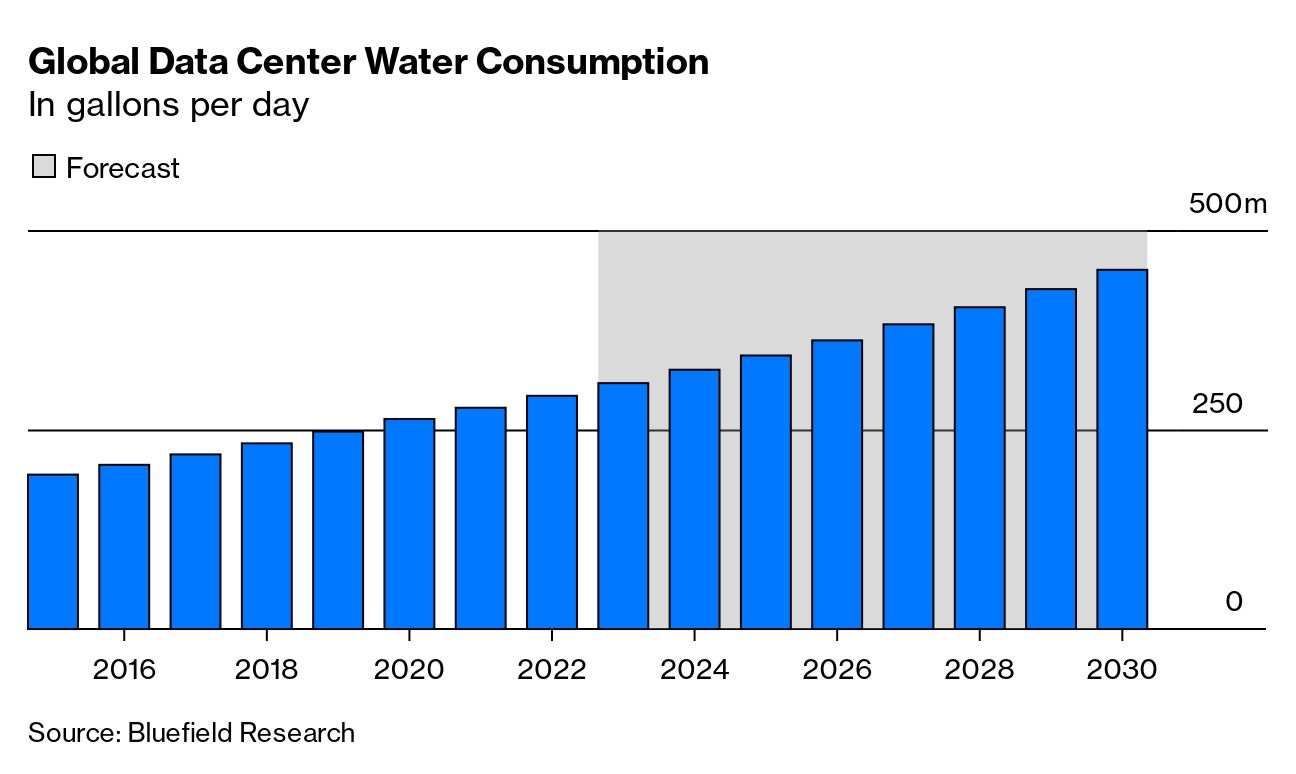
\includegraphics[width=0.8\textwidth]{pictures/water-consumption}
  \end{center}

  \begin{center}
    Data centers need (lot of) water for cooling
  \end{center}

  \begin{center}
    {\tiny (source: \url{https://siliconangle.com/2024/08/19/environmentalists-sound-alarm-virginias-data-centers-water-consumption-skyrockets/})}
  \end{center}

\end{frame}

\begin{frame}{The disaster is already here}

  \begin{center}
    The Colorado valley lost its colors!
  \end{center}

  \begin{center}
    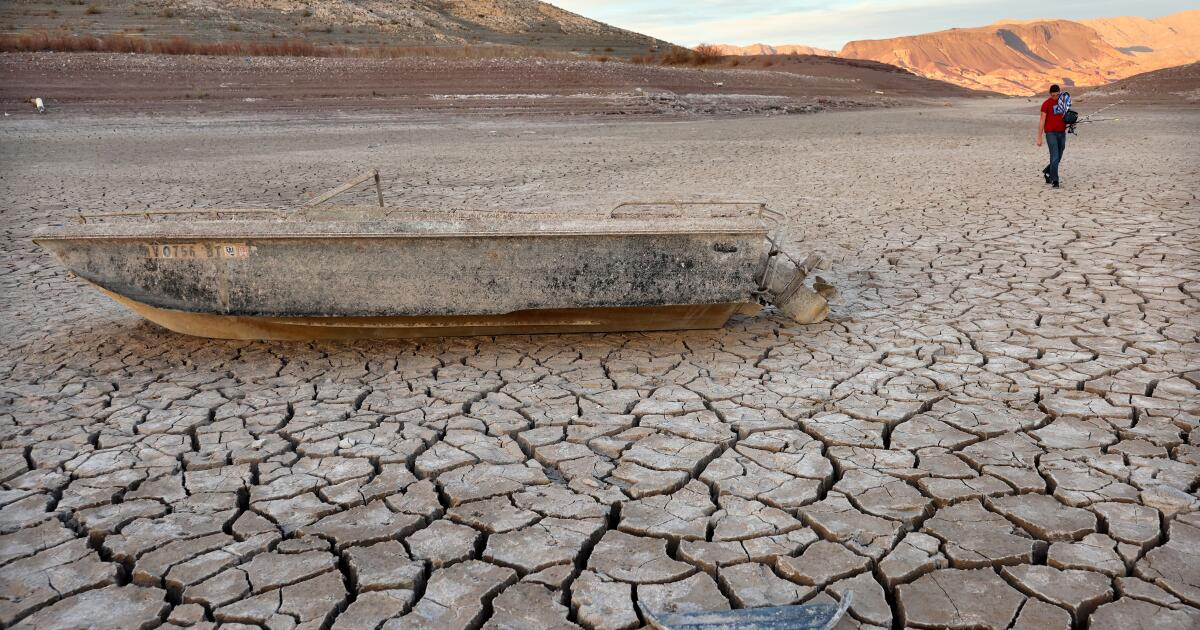
\includegraphics[width=0.75\textwidth]{pictures/colorado}
  \end{center}

\end{frame}

\begin{frame}{Not just electricity}

  \begin{center}
    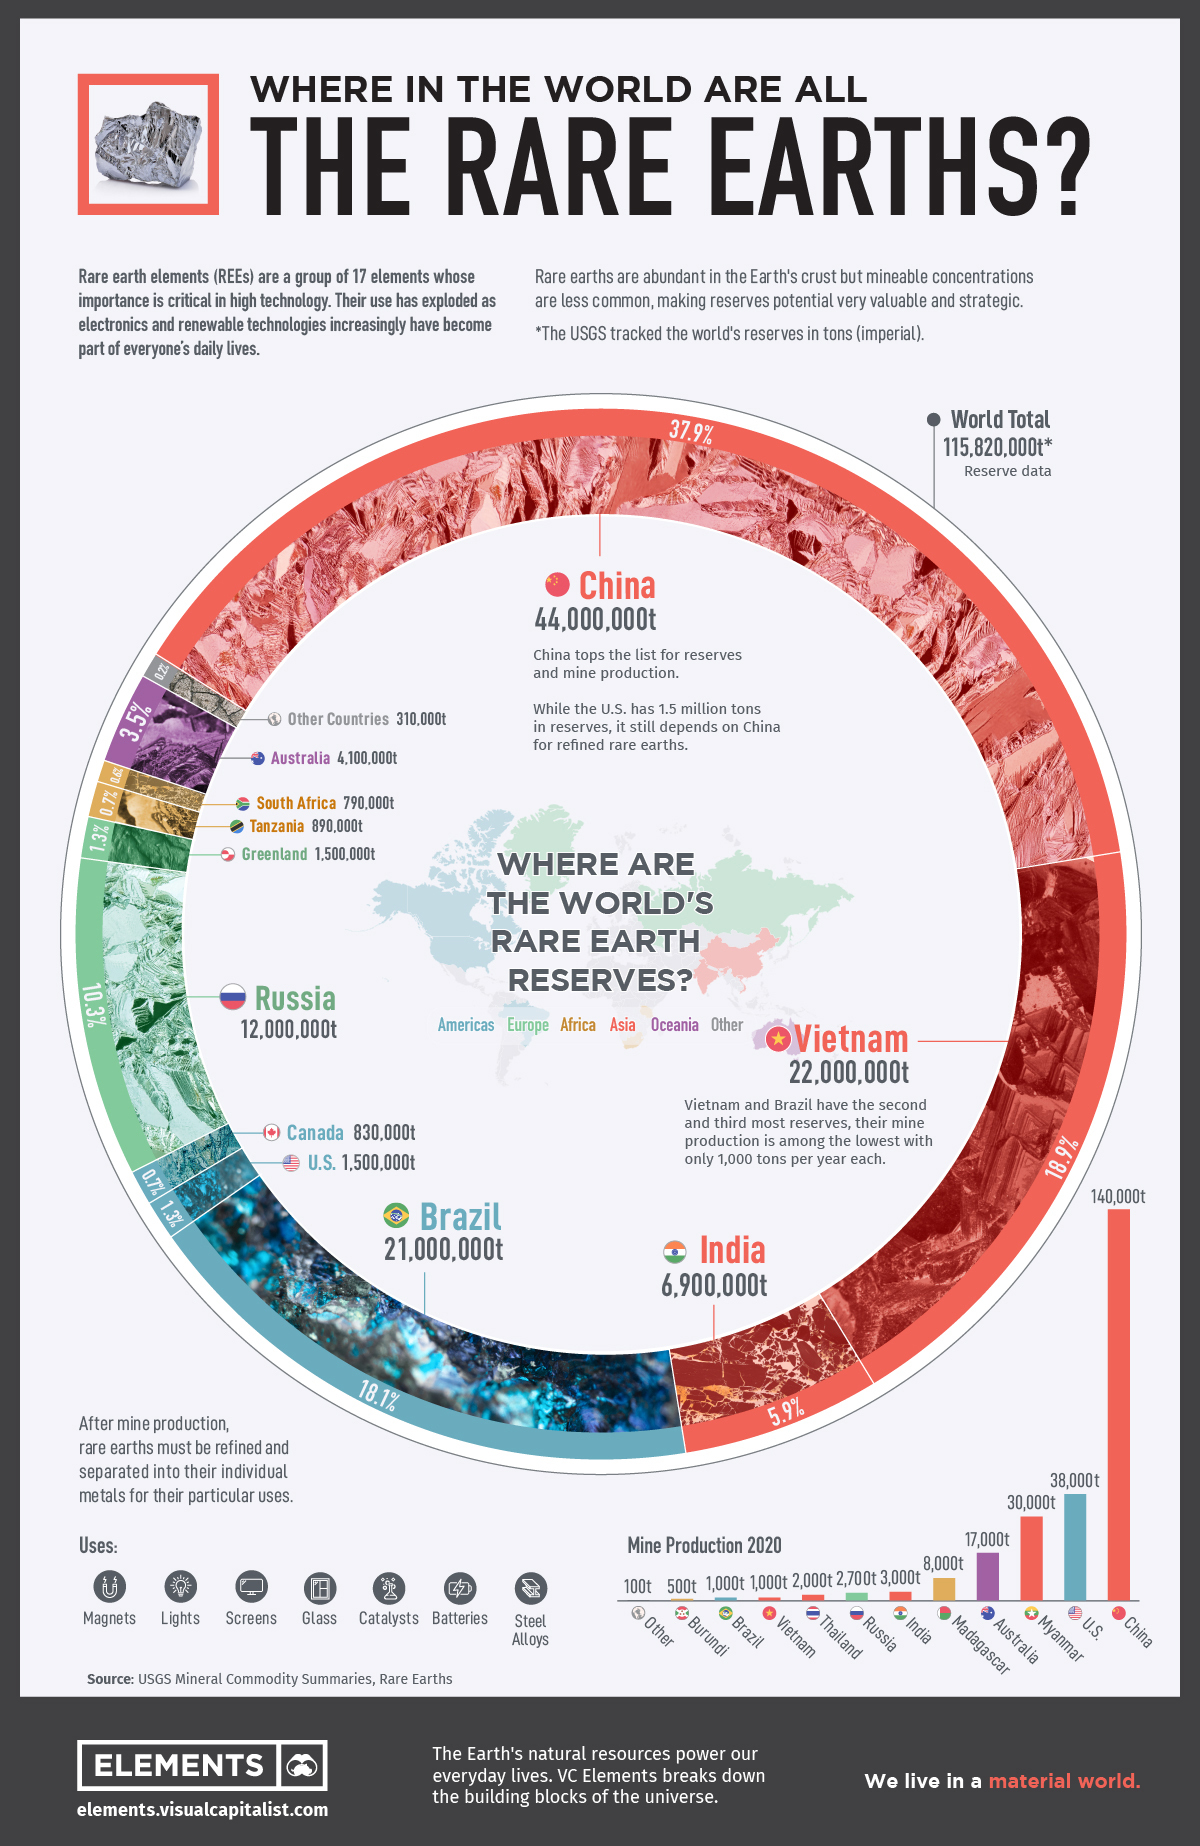
\includegraphics[width=0.42\textwidth]{pictures/rare-earths}
  \end{center}

\end{frame}

\begin{frame}{Peace and love?}

  \begin{center}
    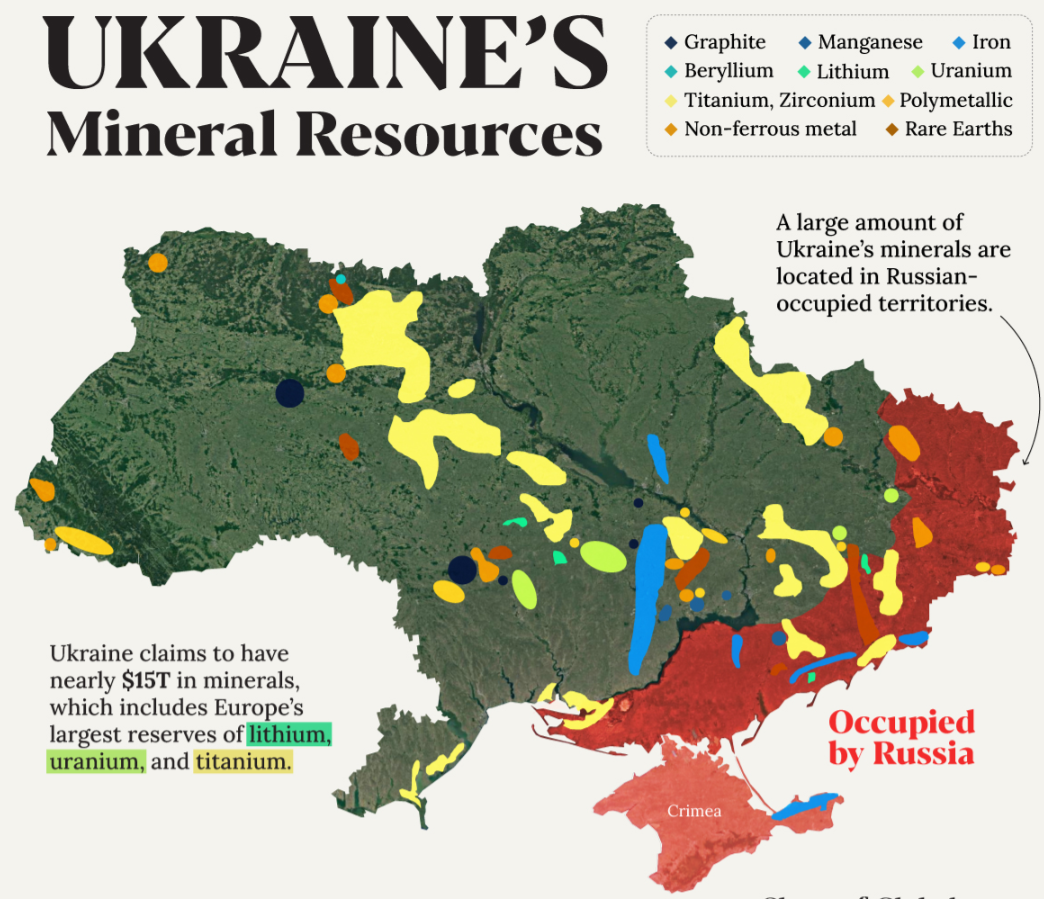
\includegraphics[width=0.7\textwidth]{pictures/ukraine}
  \end{center}

  \begin{center}
    {\tiny (source: \url{https://elements.visualcapitalist.com/mapped-ukraines-mineral-resources/})}
  \end{center}

\end{frame}

\begin{frame}{Peace and love?}

  \begin{center}
    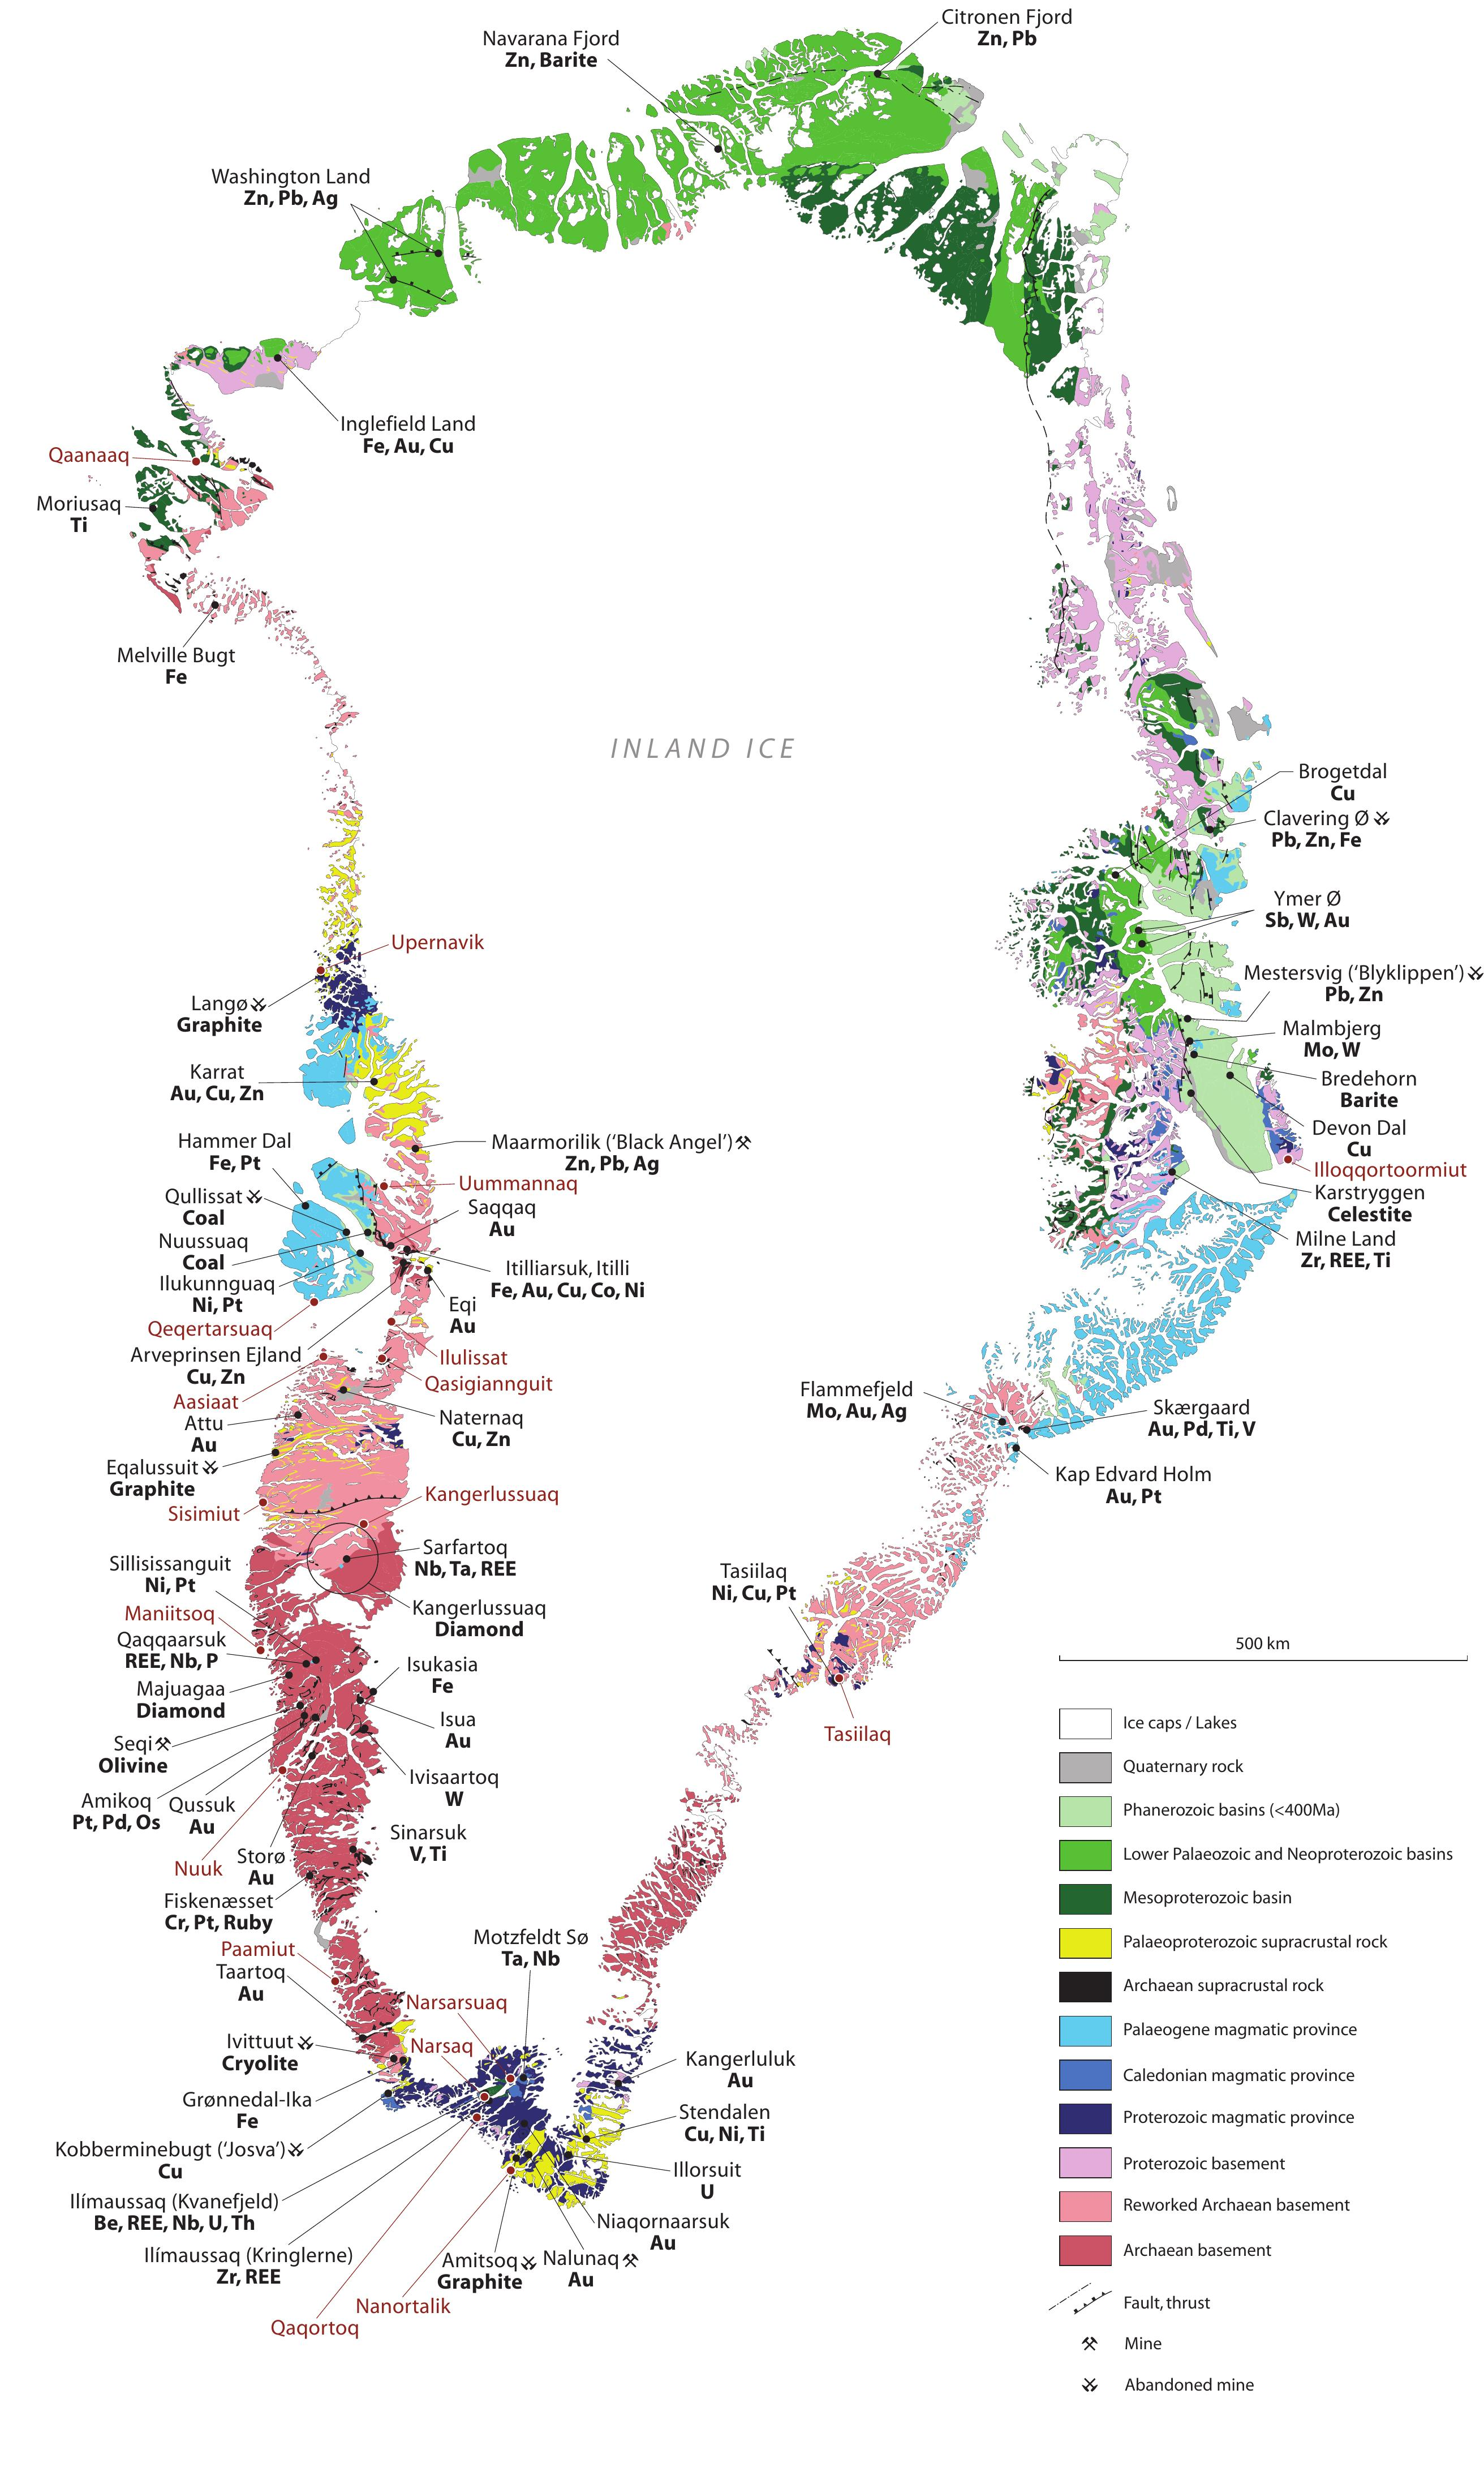
\includegraphics[width=0.35\textwidth]{pictures/greenland}
  \end{center}

  \begin{center}
    {\tiny (source: \url{https://www.academia.edu/20514876/Map_of_Greenland_geology_and_selected_mineral_occrrences})}
  \end{center}

\end{frame}

\begin{frame}{e-Waste}

  \begin{center}
    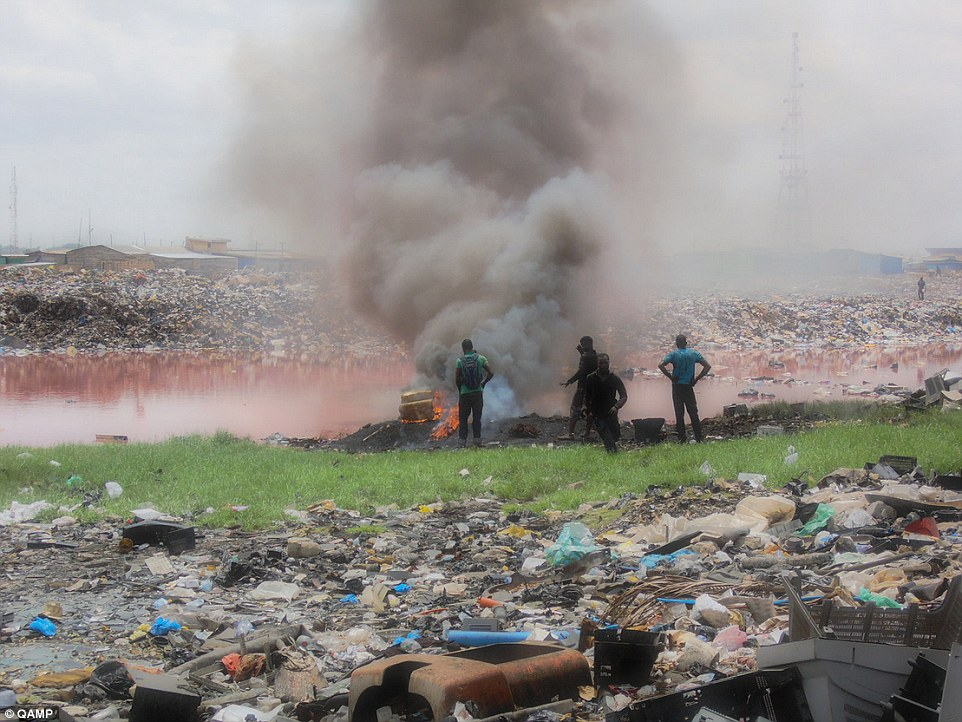
\includegraphics[width=0.7\textwidth]{pictures/e-waste}
  \end{center}

  \begin{center}
    Recycled, dumped, burned (mostly in poor countries)
  \end{center}

\end{frame}

\begin{frame}{Solutions?}

  Taming the ecological footprint of IT can only be achieved
  through a combined approach that integrates all its diverse aspects:

  \begin{itemize}
  \item technological advances
  \item social conscience
  \item political choices
  \end{itemize}

  \bigskip

  The rest of this presentation can only focus on the specific case of
  cryptocurrency mining

\end{frame}

\begin{frame}{Cryptocurrencies}
  Cryptocurrencies are one of the applications of blockchain technology:
  \begin{itemize}
  \item decentralized money (Bitcoin, Ethereum, Cardano, Solana\ldots)
  \item decentralized smart contracts
  \item decentralized identities
  \item decentralized elections
  \item decentralized supply chains
  \item \ldots
  \end{itemize}
\end{frame}

\begin{frame}{The blockchain peer-to-peer network}

  \begin{center}
    \begin{tikzpicture}[scale=0.5,>=Stealth]
      \draw[thick] (-10,0) -- (0,3.5) -- (10,0) -- cycle;

      \draw (-10,0) node[above=0.2] {\computer} node[below=0.2,fill=faustocolor] {Fausto};
      \only<2>{\draw (-7.5,1.7) node[above] {\leftArrow};}
      \only<2>{\draw (-6,2.5) node[above] {{\tiny\signature\ Alice $\xRightarrow{100}$ Donald}};}
      \draw (-10.5,3.5) rectangle +(1,0.5) [fill=gray!30!white];
      \draw[->] (-10,4.5) -- +(0,-0.5);
      \draw (-10.5,4.5) rectangle +(1,0.5) [fill=pink!70!white];
      \draw[->] (-10,5.5) -- +(0,-0.5); 
      \draw (-10.5,5.5) rectangle +(1,0.5) [fill=blue!30!white];
      \only<3->{\draw[->] (-10,6.5) -- +(0,-0.5); 
        \draw (-10.5,6.5) rectangle +(1,0.5) [fill=brown!70!white];}

      \draw (10,0) node[above=0.2] {\computer} node[below=0.2,fill=bobcolor] {Bob};
      \draw (9.5,3.5) rectangle +(1,0.5) [fill=gray!30!white];
      \draw[->] (10,4.5) -- +(0,-0.5);
      \draw (9.5,4.5) rectangle +(1,0.5) [fill=pink!70!white];
      \draw[->] (10,5.5) -- +(0,-0.5); 
      \draw (9.5,5.5) rectangle +(1,0.5) [fill=blue!30!white];
      \only<3->{\draw[->] (10,6.5) -- +(0,-0.5); 
        \draw (9.5,6.5) rectangle +(1,0.5) [fill=brown!70!white];}

      \draw[->] (0,3.5) node[above=0.2] {\computer} node[below=0.2,fill=alicecolor] {Alice};
      \only<4>{\filldraw [fill=gray!10!white] (0,8.25) circle [radius=1,very thick];}
      \only<2>{\draw (2.5,3.7) node[above] {\leftArrow};}
      \only<2>{\draw (4,4.5) node[above] {{\tiny\signature\ Donald $\xRightarrow{2500}$ John}};}
      \draw (-0.5,7) rectangle +(1,0.5) [fill=gray!30!white];
      \draw[->] (0,8) -- +(0,-0.5);
      \draw (-0.5,8) rectangle +(1,0.5) [fill=pink!70!white];
      \draw[->] (0,9) -- +(0,-0.5);
      \draw (-0.5,9) rectangle +(1,0.5) [fill=blue!30!white];
      \visible<3->{\draw[->] (0,10) -- +(0,-0.5); 
        \draw (-0.5,10) rectangle +(1,0.5) [fill=brown!70!white];}

    \end{tikzpicture}
  \end{center}

  \begin{center}
    \only<1>{Each peer holds a private copy of the same blockchain data structure}
    \only<2>{Users can send signed transactions to any peer}
    \only<3>{Such transactions get eventually boxed into new blocks}
    \only<4>{Let us inspect a block of the blockchain}
  \end{center}

\end{frame}

\begin{frame}{Blocks}
  \begin{center}
    \begin{tikzpicture}[scale=0.9]
      \visible<2->{\draw [decorate,decoration={brace,amplitude=4pt},thick,xshift=0.3cm,yshift=0pt]
        (4.5,6.5) -- (4.5,4.5) node [midway,right,xshift=.2cm] {trunk};}
      \only<1-13,15->{\draw [fill=VioletRed, thick] (0,5.5) rectangle +(4.5,1);}
      \only<14>{\shadedraw [inner color=VioletRed,outer color=white, draw=black, thick] (0,5.5) rectangle +(4.5,1);}
      \draw (2.25,6) node{height};
      \draw [fill=VioletRed, thick] (0,4.5) rectangle +(4.5,1);
      \visible<2->{\draw (2.25,5) node{$\pi$ (creator's key)};}
      \only<1-12,14->{\draw [fill=Yellow, thick] (0,3.5) rectangle +(4.5,1);}
      \only<13>{\draw [inner color=Yellow,outer color=white, draw=black, thick] (0,3.5) rectangle +(4.5,1);}
      \only<3->{\draw (2.25,4) node{$\previousblockhash$};}
      \only<-3>{\phantom{\draw[->,thick] (0,4) -- (-1,4) node [midway,left,xshift=-.5cm] {$\previous$};}}
      \only<3->{\draw[->,thick] (0,4) -- (-1,4) node [midway,left,xshift=-.5cm] {$\previous$};}

      \draw [fill=Yellow, thick] (0,2.5) rectangle +(4.5,1);
      \visible<4->{\draw (2.25,3) node{nonce\,(arbitrary\,number)};}
      \only<1-14,17->{\draw [fill=Yellow, thick] (0,1.5) rectangle +(4.5,1);}
      \only<15,16>{\draw [inner color=Yellow,outer color=white, draw=black, thick] (0,1.5) rectangle +(4.5,1);}
      \visible<5->{\draw (2.25,2) node{$\tau$ (creation time)};}

      \only<1-6,8-16>{\draw [fill=SpringGreen, thick] (0,-1) rectangle +(4.5,2.5);}
      \only<7,17,18>{\draw [inner color=SpringGreen,outer color=white, draw=black, thick] (0,-1) rectangle +(4.5,2.5);}
      \visible<6-7>{\draw (2.25,0.3) node{transactions};}
      \visible<8->{\draw (2.25,1.1) node{\signature\ Alice $\xRightarrow{100}$ Donald};}
      \visible<9->{\draw (2.25,0.5) node{\signature\ Fausto $\xRightarrow{500}$ John};}
      \visible<10->{\draw (2.25,-0.1) node{\signature\ Donald $\xRightarrow{350}$ Alice};}
      \visible<11->{\draw (2.25,-0.7) node{\signature\ Donald $\xRightarrow{2500}$ John};}
    \end{tikzpicture}
  \end{center}

  \begin{center}
    \only<1-6>{\phantom{Rule 2: $\previous$ actually exists (no dangling pointers)}}
    \only<7-11>{Let us inspect the list of transactions}
    \only<12>{Valid blocks satisfy all \alert{consensus rules}}
    \only<13>{\alert{Rule 1:} $\previous$ actually exists (no dangling pointers)}
    \only<14>{\alert{Rule 2:} The height increases: $\height=\previous.\height+1$}
    \only<15>{\alert{Rule 3:} The creation time increases: $\previous.\tau<\tau$}
    \only<16>{\alert{Rule 4:} The creation time is not in the future: $\tau\le\tau_\now$}
    \only<17>{\alert{Rule 5:} Each transaction is correctly signed by its sender}
    \only<18>{\alert{Rule 6:} Senders hold the money that they send}
  \end{center}

\end{frame}

\begin{frame}{Each peer (Alice) can expand a \textbf{block} with a \textbf{next} block}

  \begin{center}
    \begin{tikzpicture}[scale=0.9]
      \draw (2,7) node{\textbf{block}};
      \draw [fill=VioletRed, thick] (0,4.5) rectangle (4,6.5);
      \draw (2,6) node{height};
      \draw [fill=VioletRed, thick] (0,3.5) rectangle (4,5.5);
      \draw (2,5) node{$\pi$ (creator's key)};
      \draw [fill=Yellow, thick] (0,3.5) rectangle (4,4.5);
      \draw (2,4) node{$\previousblockhash$};

      \draw [fill=Yellow, thick] (0,2.5) rectangle (4,3.5);
      \draw (2,3) node{nonce};
      \draw [fill=Yellow, thick] (0,1.5) rectangle (4,2.5);
      \draw (2,2) node{$\tau$ (creation time)};

      \draw [fill=SpringGreen, thick] (0,-1) rectangle (4,1.5);
      \draw (2,0.25) node{transactions};

      \visible<2->{
      \draw (9,7) node{\textbf{next}};
      \draw [fill=VioletRed, thick] (6,5.5) rectangle (12,6.5);
      \draw (9,6) node{height+1};
      }
      \visible<3->{
      \draw [fill=VioletRed, thick] (6,4.5) rectangle (12,5.5);
      \draw (9,5) node{Alice's public key};
      }
      \visible<4->{
      \draw [fill=Yellow, thick] (6,3.5) rectangle (12,4.5);
      \draw (9,4) node{$\hash(\mathbf{block})$};
      \draw[->,very thick] (6,4) -- (4,4);
      }

      \visible<5->{
      \draw [fill=Yellow, thick] (6,2.5) rectangle (12,3.5);
      \draw (9,3) node{42 (or 17, or 13, or your bday)};
      }
      \visible<6->{
      \draw [fill=Yellow, thick] (6,1.5) rectangle (12,2.5);
      \draw (9,2) node{$\tau_\now$};
      }

      \visible<7->{
      \draw [fill=SpringGreen, thick] (6,-1) rectangle (12,1.5);
      \draw (9,1) node{\signature\ Alice $\xRightarrow{100}$ Donald};
      \draw (9,0.25) node{\signature\ Donald $\xRightarrow{2500}$ John};
      }

      \visible<8->{
      \draw (9,-0.5) node{\textbf{ $\xRightarrow{432}$ Alice}};
      }
    \end{tikzpicture}
  \end{center}

\end{frame}

\begin{frame}{Peers create (``mine'') new blocks}

  \begin{center}
    \begin{tikzpicture}[scale=0.5,>=Stealth]

      \draw[thick] (-10,0) -- (0,3.5) -- (10,0) -- cycle;

      \draw (-10,0) node[above=0.2] {\computer} node[below=0.2,fill=faustocolor] {Fausto};
      \draw (-10.5,3.5) rectangle +(1,0.5) [fill=gray!30!white];
      \draw[->] (-10,4.5) -- +(0,-0.5);
      \draw (-10.5,4.5) rectangle +(1,0.5) [fill=pink!70!white];
      \draw[->] (-10,5.5) -- +(0,-0.5); 
      \draw (-10.5,5.5) rectangle +(1,0.5) [fill=blue!30!white];
      \visible<2-3,5,7-8,10>{\draw[->] (-10,6.5) -- +(0,-0.5);}
      \visible<9>{\draw[->] (-10.5,6.5) -- +(0.5,-0.5);}
      \visible<9>{\draw[->] (-9.5,6.5) -- +(-0.5,-0.5);}
      \visible<2-3,8>{\draw (-10.5,6.5) rectangle +(1,0.5) [fill=faustocolor];}
      \visible<5,10>{\draw (-10.5,6.5) rectangle +(1,0.5) [fill=alicecolor];}
      \visible<7>{\draw (-10.5,6.5) rectangle +(1,0.5) [fill=bobcolor];}
      \visible<9>{\draw (-11.2,6.5) rectangle +(1,0.5) [fill=faustocolor];}
      \visible<9>{\draw (-9.8,6.5) rectangle +(1,0.5) [fill=alicecolor];}

      \draw (10,0) node[above=0.2] {\computer} node[below=0.2,fill=bobcolor] {Bob};
      \draw (9.5,3.5) rectangle +(1,0.5) [fill=gray!30!white];
      \draw[->] (10,4.5) -- +(0,-0.5);
      \draw (9.5,4.5) rectangle +(1,0.5) [fill=pink!70!white];
      \draw[->] (10,5.5) -- +(0,-0.5); 
      \draw (9.5,5.5) rectangle +(1,0.5) [fill=blue!30!white];
      \visible<3,5-7,10>{\draw[->] (10,6.5) -- +(0,-0.5);}
      \visible<9>{\draw[->] (9.5,6.5) -- +(0.5,-0.5);}
      \visible<9>{\draw[->] (10.5,6.5) -- +(-0.5,-0.5);}
      \visible<3>{\draw (9.5,6.5) rectangle +(1,0.5) [fill=faustocolor];}
      \visible<5,10>{\draw (9.5,6.5) rectangle +(1,0.5) [fill=alicecolor];}
      \visible<6-7>{\draw (9.5,6.5) rectangle +(1,0.5) [fill=bobcolor];}
      \visible<9>{\draw (8.8,6.5) rectangle +(1,0.5) [fill=faustocolor];}
      \visible<9>{\draw (10.2,6.5) rectangle +(1,0.5) [fill=alicecolor];}

      \draw (0,3.5) node[above=0.2] {\computer} node[below=0.2,fill=alicecolor] {Alice};
      \draw (-0.5,7) rectangle +(1,0.5) [fill=gray!30!white];
      \draw[->] (0,8) -- +(0,-0.5);
      \draw (-0.5,8) rectangle +(1,0.5) [fill=pink!70!white];
      \draw[->] (0,9) -- +(0,-0.5);
      \draw (-0.5,9) rectangle +(1,0.5) [fill=blue!30!white];
      \visible<3-5,7-8,10>{\draw[->] (0,10) -- +(0,-0.5);}
      \visible<9>{\draw[->] (-0.5,10) -- +(0.5,-0.5);}
      \visible<9>{\draw[->] (0.5,10) -- +(-0.5,-0.5);}
      \visible<3>{\draw (-0.5,10) rectangle +(1,0.5) [fill=faustocolor];}
      \visible<4-5,8,10>{\draw (-0.5,10) rectangle +(1,0.5) [fill=alicecolor];}
      \visible<7>{\draw (-0.5,10) rectangle +(1,0.5) [fill=bobcolor];}
      \visible<9>{\draw (-1.2,10) rectangle +(1,0.5) [fill=faustocolor];}
      \visible<9>{\draw (0.2,10) rectangle +(1,0.5) [fill=alicecolor];}

    \end{tikzpicture}
  \end{center}

  \begin{overprint}
    \onslide<2-3>
    \centering Fausto creates a new block\ldots
    \onslide<4-5>
    \centering \ldots or Alice creates a new block
    \onslide<6-7>
    \centering \ldots or Bob creates a new block
    \onslide<8-9>
    \centering \ldots or Fausto and Alice create a new block!
    \onslide<10>
    \centering Peers select the block with the largest hash
  \end{overprint}

\end{frame}

\begin{frame}{Blockchain mining as a competitive puzzle}

  Mining of a \textbf{next} block on top of a \textbf{block}:
  \quad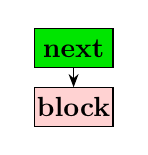
\begin{tikzpicture}[scale=0.5,>=Stealth]
    \draw (0,1.5) rectangle +(2,1) [fill=alicecolor];
    \draw[->] (1,1.5) -- +(0,-0.5);
    \draw (0,0) rectangle +(2,1) [fill=pink!70!white];
    \draw (1,0) node[above] {\textbf{block}};
    \draw (1,1.5) node[above] {\textbf{next}};
  \end{tikzpicture}

  \begin{description}
  \item[{\color{red}challenge:}] \only<2->{derive (deterministically) a challenge from the \textbf{block}}
  \item[{\color{red}answer:}] \only<3->{send all peers a \textbf{next} that satisfies the challenge}
  \item[{\color{red}competition:}] \only<4->{in case of more \textbf{next}, select a \emph{best} one}
  \end{description}

  \bigskip
  \visible<5->{Bitcoin's Proof of Work (PoW):}
  \begin{description}
  \item<6->[{\color{red}challenge:}] find a \textbf{next}, with backwards pointer $\hash(\mathbf{block})$,
    such that $\hash(\mathbf{next})>\difficulty$
  \item<7->[{\color{red}answer:}] send all peers a \textbf{next}, with backwards pointer $\hash(\mathbf{block})$, obtained
    by rotating among possible values for the nonce of $\mathbf{next}$, until $\hash(\mathbf{next})>\difficulty$
  \item<8->[{\color{red}competition:}] in case of more \textbf{next}, select the one with the largest hash
  \end{description}

\end{frame}

\begin{frame}[fragile]{Bitcoin's proof of work mining is brute force}
 
\begin{algorithm}[H] 
\caption{Bitcoin's Proof of Work}
\begin{algorithmic}[1]
\Require{$block$, $difficulty$, $max$} 
\Ensure{$next$ (a valid child of $block$, or null)}
\Statex
\State {$next$ $\gets$ null}
\For{$nonce \gets 0$ to $max$}
\State {$candidate$ $\gets$ valid block pointing back to $block$ and using $nonce$}
\If{hash($candidate$) $\ge$ $difficulty$}
\If{$next$ = null \textbf{or} hash($candidate$) $>$ hash($next$)}
\State {$next$ $\gets$ $candidate$}
\EndIf
\EndIf
\EndFor
\State \Return {$next$}
\end{algorithmic}
\end{algorithm} 

\end{frame}

\begin{frame}\frametitle{Evolution of Bitcoin's mining hardware}

  \begin{center}
    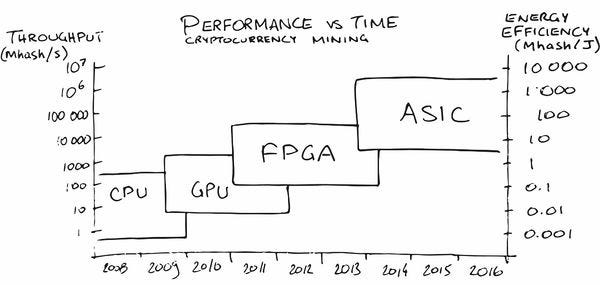
\includegraphics[scale=0.55,clip=false]{pictures/mining-hardware}
  \end{center}

\end{frame}

\begin{frame}\frametitle{Bitcoin's difficulty over the years}

  \begin{center}
    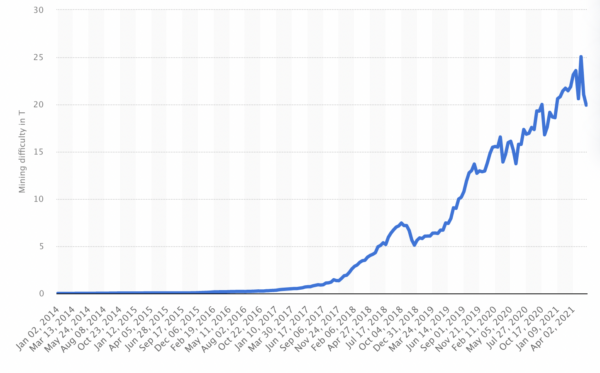
\includegraphics[width=0.9\textwidth,clip=false]{pictures/difficulty}
  \end{center}

  \begin{center}
    {\tiny (source: \url{https://thresh0ld.com/bitcoin-mining-difficulty-and-price-correlation})}
  \end{center}
    
\end{frame}

\begin{frame}\frametitle{Bitcoin's energy consumption over the years}

  \begin{center}
    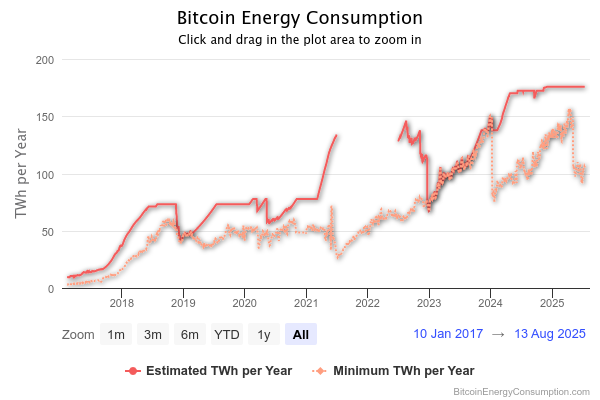
\includegraphics[width=0.9\textwidth,clip=false]{pictures/bitcoin-energy-consumption}
  \end{center}

  \begin{center}
    {\tiny (source: \url{https://digiconomist.net/bitcoin-energy-consumption})}
  \end{center}

\end{frame}

\begin{frame}\frametitle{Annualized Bitcoin's total footprint}

  \begin{center}
    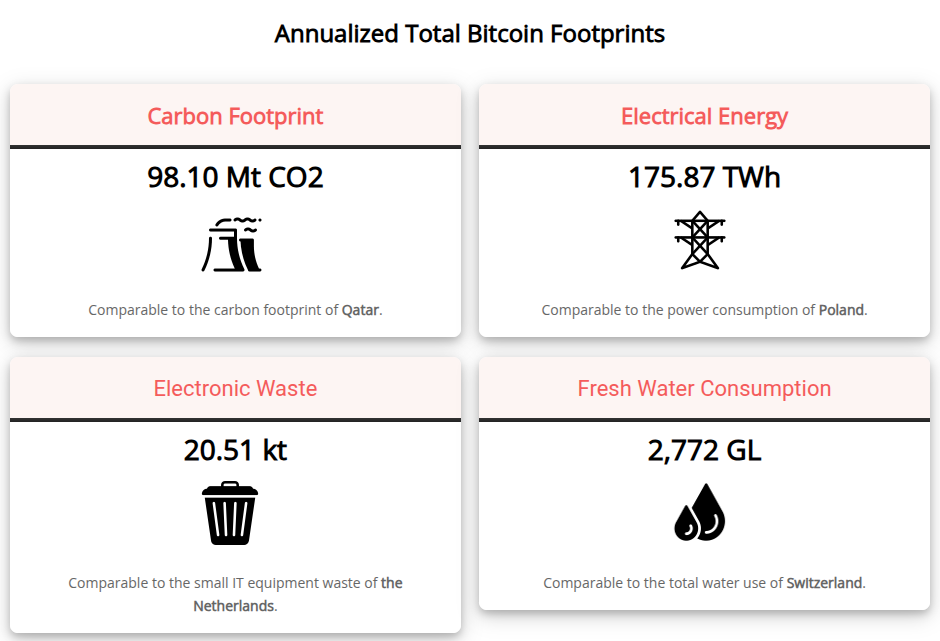
\includegraphics[width=0.85\textwidth,clip=false]{pictures/footprint-annual}
  \end{center}

  \begin{center}
    {\tiny (source: \url{https://digiconomist.net/bitcoin-energy-consumption})}
  \end{center}

\end{frame}

\begin{frame}\frametitle{Bitcoin's footprint for a single transaction}

  \begin{center}
    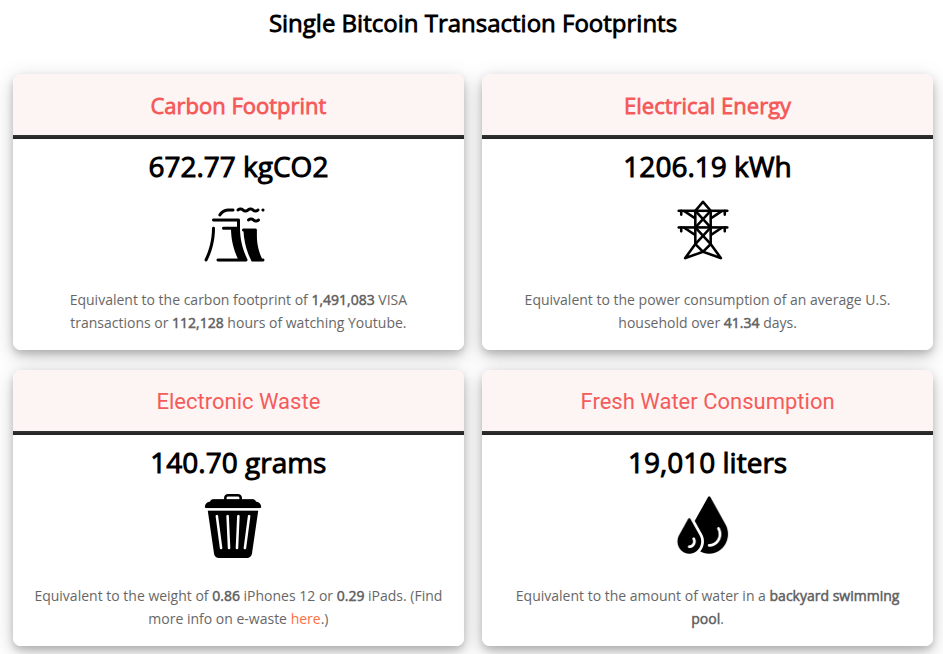
\includegraphics[width=0.85\textwidth,clip=false]{pictures/footprint-single}
  \end{center}

  \begin{center}
    {\tiny (source: \url{https://digiconomist.net/bitcoin-energy-consumption})}
  \end{center}

\end{frame}

\begin{frame}\frametitle{The proof of stake approach}

  \begin{center}
    Jae Kwon, \emph{Tendermint, Consensus without Mining}, 2014
  \end{center}

  \begin{greenbox}{}
    A selected set of peers (\emph{validators}) decide the next blocks, in
    a round robin way or according to any other \emph{fair} policy, typically
    based on the amount of money \emph{staked} by each validator.
    Byzantine algorithms ensure the survival of the peer-to-peer network if
    some validator misbehaves.
  \end{greenbox}

  \medskip

  \begin{center}
    Pros: no CPU mining anymore, higher throughput
  \end{center}

  \begin{center}
    Cons: more centralized, the rich become richer
  \end{center}

  \begin{center}
    $99\%$ of cryptocurrencies are based on proof of stake nowadays
  \end{center}

  \pause

  \begin{center}
    \alert{Are Bitcoin and its proof of work dead then?}
  \end{center}

\end{frame}

\begin{frame}{It's the economy, stupid!}

  \begin{center}
    Bitcoin (proof of work) to USD\\
    \vspace*{1ex}
    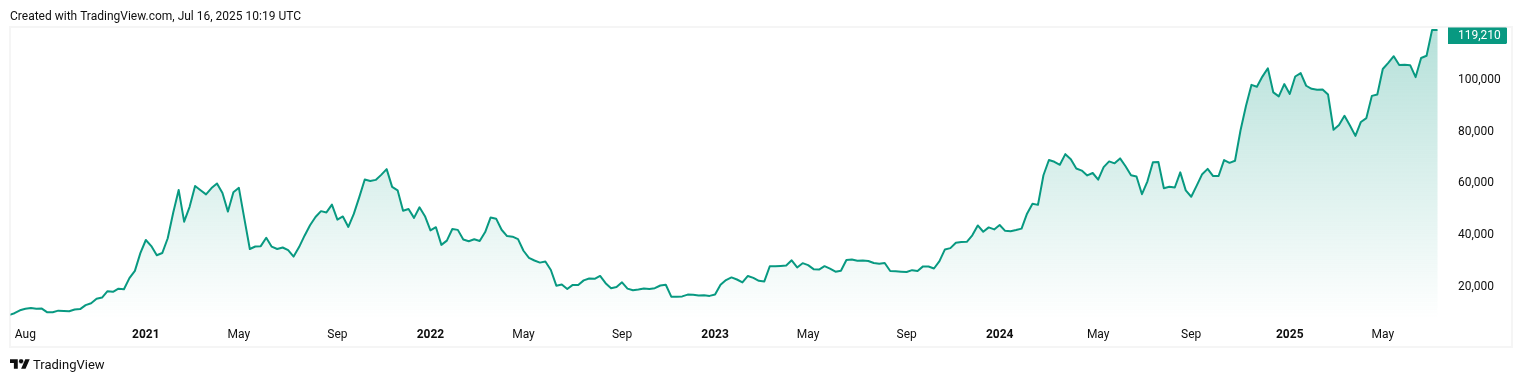
\includegraphics[width=\textwidth]{pictures/BTCUSD}
  \end{center}

  \medskip

  \begin{overprint}
    \onslide<2>
    \begin{center}
      Ethereum (proof of stake) to USD\\
      \vspace*{1ex}
      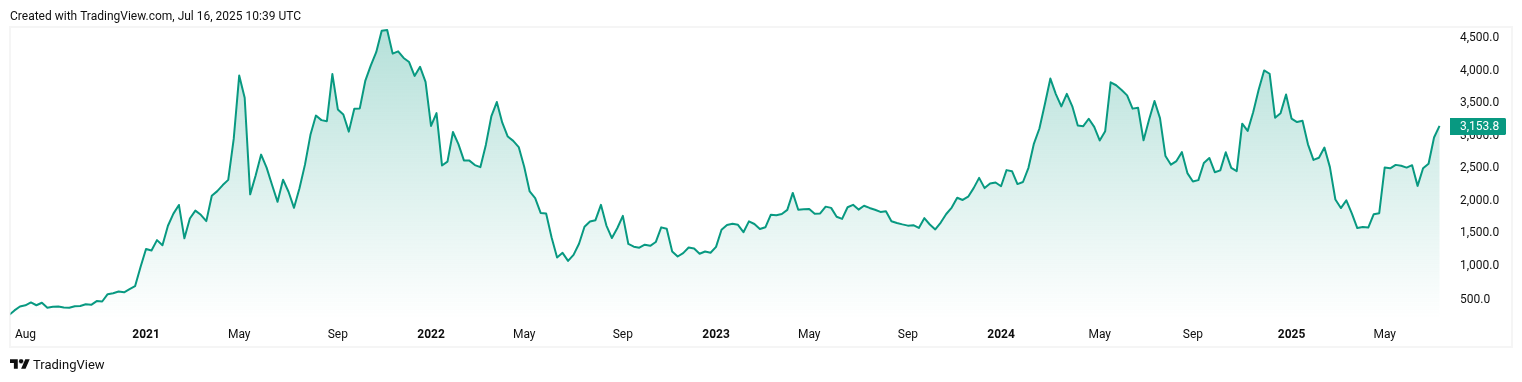
\includegraphics[width=\textwidth]{pictures/ETHUSD}
    \end{center}
    \onslide<3>
    \begin{center}
      Solana (proof of stake) to USD\\
      \vspace*{1ex}
      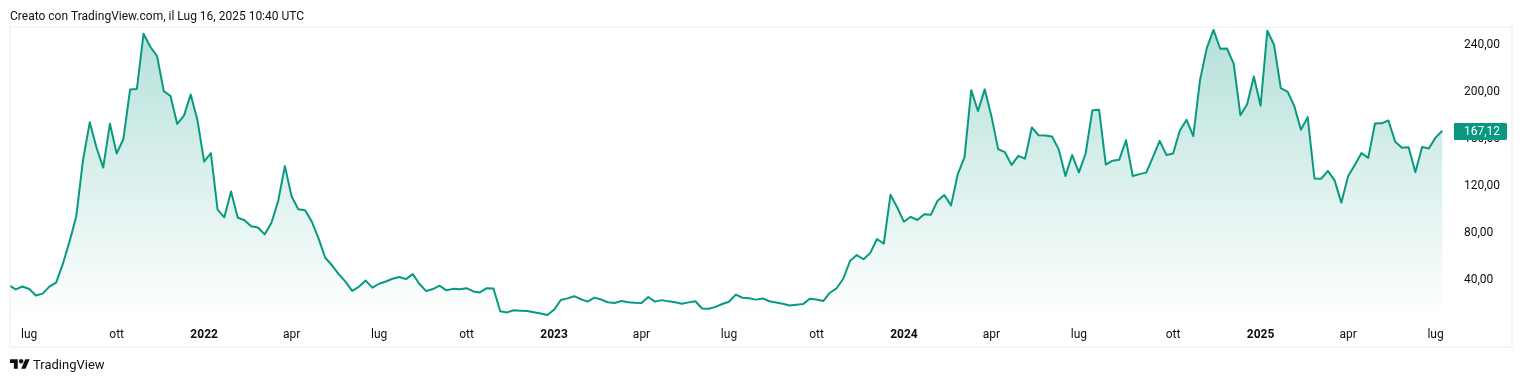
\includegraphics[width=\textwidth]{pictures/SOLUSD}
    \end{center}
    \onslide<4>
    \begin{center}
      Cardano (proof of stake) to USD\\
      \vspace*{1ex}
      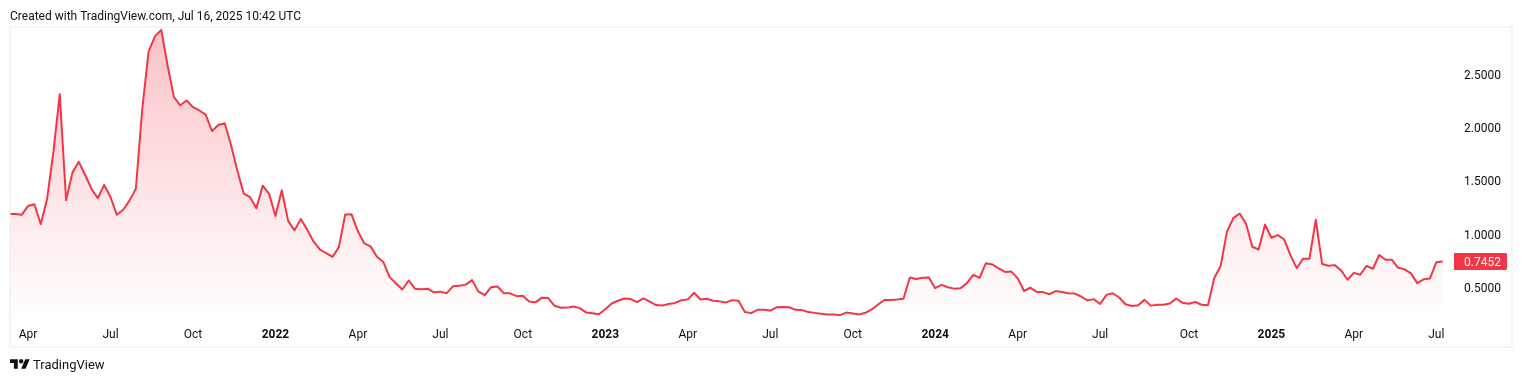
\includegraphics[width=\textwidth]{pictures/ADAUSD}
    \end{center}
    \onslide<5>
    \begin{center}
      Polygon (proof of stake) to USD\\
      \vspace*{1ex}
      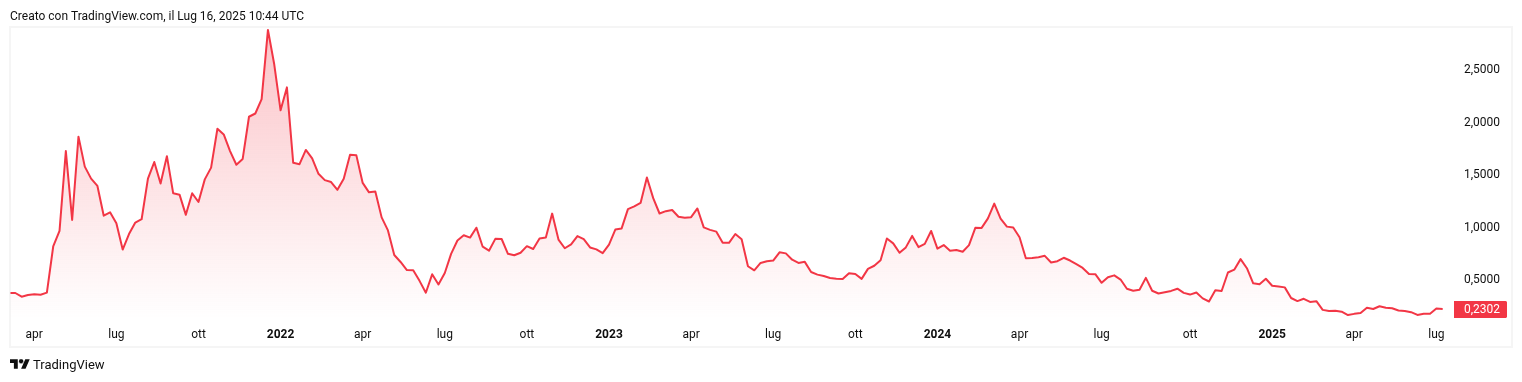
\includegraphics[width=\textwidth]{pictures/MATICUSD}
    \end{center}
    \centering \ldots or Fausto and Alice create a new block!
    \onslide<6>
    \begin{center}
      Dogecoin (proof of stake) to USD\\
      \vspace*{1ex}
      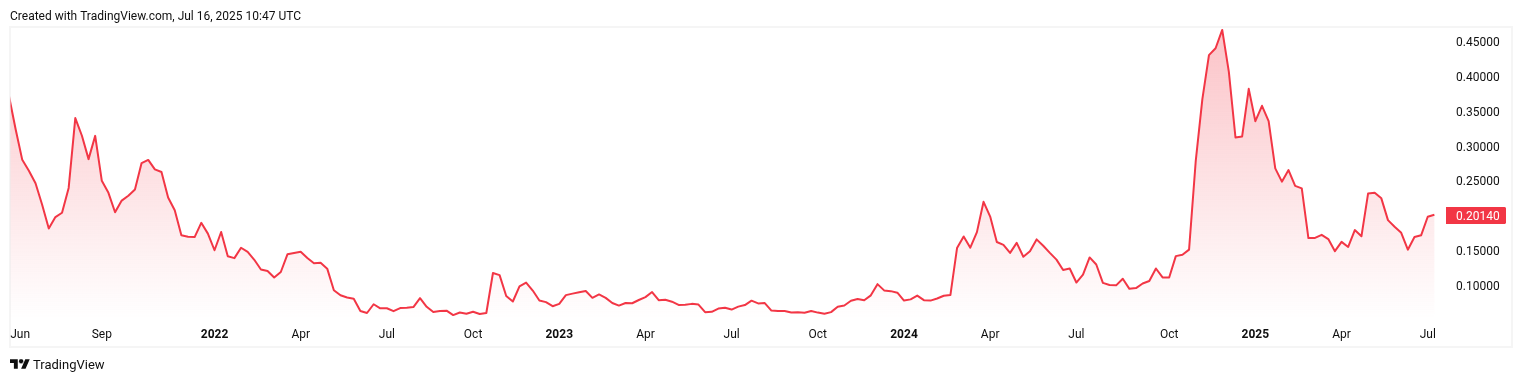
\includegraphics[width=\textwidth]{pictures/DOGEUSD}
    \end{center}
  \end{overprint}

\end{frame}

\begin{frame}{Looking for the chimera}

  \begin{center}
    As decentralized as Bitcoin's proof of work, as cheap as proof of stake
  \end{center}

  \medskip

  \begin{center}
    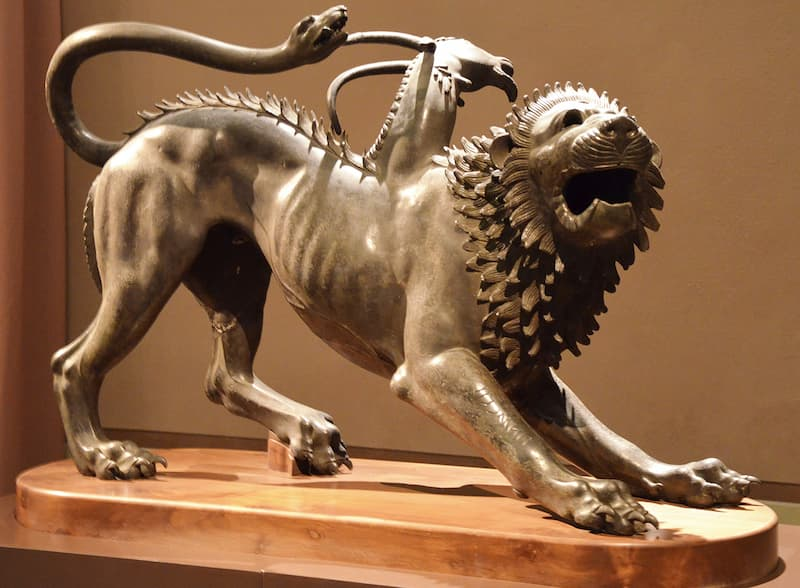
\includegraphics[width=0.7\textwidth]{pictures/chimera}\\
    {\tiny Florence, Etruscan chimera, 400 BC}
  \end{center}

\end{frame}

\begin{frame}{An email from \texttt{crypto42@pm.me} (September 30, 2021)}

  \begin{greenbox}{}
    Hi Fausto!

    \vspace{2ex}

    I have been experimenting with a blockchain called \alert{Signum: \url{https://signum.network/}}.
    They \alert{mine with
    disk drive files (plot files)}, which is far more at reach
    and \alert{ecological} than GPUs or CPUs.

    \vspace{1ex}

    I've been trying with other developers to make their mining 100\%
    Java based. This would open the door for end-users to easily \alert{mine directly
    from their cellphones} or from low-powered devices fueled by \alert{green energy}.
    Unfortunately that was beyond our skills.

    \vspace{1ex}

    I saw your Hotmoka smart contracts project on GitHub.
    I wonder if disk drive mining, also on cell phones, can be achieved with Hotmoka.
  \end{greenbox}

\end{frame}

\begin{frame}{What I could learn about Signum}

  \begin{itemize}
  \item very simple protocol for proof of space (PoSp)
  \item running since 2014 (as Burstcoin)
  \item possibly the first ever smart contracts (before Ethereum!)
  \item proof of space (they call it proof of capacity)
  \item recently, proof of space + proof of commitment
    \begin{itemize}
    \item[] just a factor multiplication of proof of space
      based on the committed cryptocurrency, as an incentive
      to buying their cryptocurrency
    \end{itemize}
  \item commercial web page: \url{https://signum.network/}
  \item very informal documentation:
    \url{https://wiki.signum.network}
  \item chaotic, uncommented, monolithic code:
    \url{https://github.com/signum-network/signum-node}
  \item Park et al., \emph{SpaceMint: A Cryptocurrency Based on Proofs of Space},
    Financial Cryptography 2018,
    show that Signum originally suffered from a time/memory tradeoff
    and suspect that it suffers from block-grinding attacks as well
  \end{itemize}

\end{frame}

\begin{frame}\frametitle{Proof of space is much more than Signum}

  \begin{greenbox}{}
    \begin{itemize}
    \item Ateniese, Bonacina, Faonio, Galesi: \emph{Proofs of Space: When Space Is of the Essence}, 2014 (DAG pebbling)
    \item Dziembowski, Faust, Kolmogorov, Pietrzak: \emph{Proofs of Space}, 2015 (DAG pebbling) $\Rightarrow$
      {\color{red}SpaceMint}: \url{https://github.com/kwonalbert/spacemint}
    \item Abusalah, Alwen, Cohen, Khilko, Pietrzak, Reyzin: \emph{Beyond Hellman's Time-Memory Trade-Offs with Applications to Proofs of Space}, 2017 (proof of sequential work + proof of space) $\Rightarrow$ {\color{red}Chia}: \url{https://www.chia.net/wp-content/uploads/2022/07/ChiaGreenPaper.pdf}
    \item \emph{Signum Community Website and Documentation Project} (plot files) $\Rightarrow$ {\color{red}Signum}: \url{https://wiki.signum.network}
    \end{itemize}

  \begin{center}
    {\small\begin{tabular}{c|c|c|c|c|c}
      tool & consensus & network & formalized & since & status \\\hline\hline
      SpaceMint & no & no & yes & 2015 & discontinued\\\hline
      Chia & yes & yes & yes & 2017 & active\\\hline
      Signum & yes & yes & no & 2014 & active\\\hline
    \end{tabular}}
  \end{center}
  \end{greenbox}
  
\end{frame}

\begin{frame}\frametitle{Proof of space: The general idea}

  \begin{description}
  \item[Ideal PoSp:] the computation of the answer can only be achieved by allocating
    a big data structure on disk (Ateniese et al., Dziembowski et al., Abusalah et al.)
    \medskip
  \item[Signum's PoSp:] the computation of the answer can also be achieved without
    allocating a big data structure on disk (precomputed \emph{nonces}),
    but in that case it becomes
    computationally so expensive (to recompute the data on-the-fly)
    that the space of explorable data, before the next block is created, is very small
  \end{description}

  \bigskip
  
  \begin{redbox}{Time/memory trade-off}
    The degradation of the space of explorable data should be at least linear with
    the reduction of the precomputed data
  \end{redbox}

\end{frame}

\begin{frame}\frametitle{Signum's proof of space}

  \visible<1->{Blocks are enriched with a $\nonce$ data structure of size $n$ and creator $\pi$}
  \medskip

  \begin{description}
  \item<2->[{\color{red}challenge:}] given a $\challenge$
    derived from \textbf{block}, find a block \textbf{next}, with backwards pointer
    $\hash(\mathbf{block})$, with a $\nonce$ data structure for the same creator of the block,
    such that $\delay(\nonce,\challenge)$ is as smaller as possible
  \item<3->[{\color{red}answer:}] reply with a \textbf{next}, pointing back
    with $\hash(\mathbf{block})$, that contains a $\nonce$ from
    a large set of nonces precomputed on disk,
    choosing the one minimizing $\delay(\nonce,\challenge)$
    and using as block's creator the same creator of $\nonce$
  \item<4->[{\color{red}competition:}] in case of more \textbf{next}, select the one with the smallest
    $\delay(\nonce,\challenge)$
  \end{description}

\end{frame}

\begin{frame}{A work of formalization}

  A formalization of Signum's proof of space requires to clarify:
  \begin{description}
  \item[Point~1:] what is the nonce data structure
  \item[Point~2:] how a challenge is derived from a block
  \item[Point~3:] how $\delay(\nonce,\challenge)$ is defined
  \end{description}

  \pause

  \medskip

  Once a formalization is available, it can be used to \alert{prove} that
  the algorithm is immune to some typical attacks and as the basis for
  a clean implementation.

  \bigskip

  \begin{greenbox}{}
    Fausto Spoto, \emph{A Formalization of Signum Consensus},
    Financial Cryptography Workshop on Trusted Smart Contracts,
    Miyakojima, Japan, 2025, To appear in LNCS.
  \end{greenbox}

\end{frame}

\begin{frame}{Point~1: The nonce data structure}
  \begin{center}
    $p\in\mathbb{N}$ (\emph{progressive}) and $\pi\in\mathit{byte}^*$ (public key of creator)
  \end{center}
  \[\begin{array}{l}
  \pause
  \seed=\pi\bowtie p\quad\text{($\bowtie$ is byte array concatenation)}\\
  \pause
  {\color{blue} h_0}=\hashfirstk(\seed)\\
  \pause
  {\color{blue} h_1}=\hashfirstk({\color{blue} h_0}\bowtie\seed)\\
  \pause
  {\color{blue} h_2}=\hashfirstk({\color{blue} h_1}\bowtie{\color{blue}  h_0}\bowtie \seed)\\
  \pause
  \vdots\\
  {\color{blue} h_{2n-1}}=\hashfirstk({\color{blue} h_{2n-2}}\bowtie{\color{blue} h_{2n-3}}\bowtie\cdots\bowtie{\color{blue} h_1}\bowtie{\color{blue} h_0}\bowtie \seed)\\
  \pause
  {\color{red}\finalhash}=\hash({\color{blue} h_{2n-1}}\bowtie{\color{blue} h_{2n-2}}\bowtie\cdots\bowtie{\color{blue} h_1}\bowtie{\color{blue} h_0}\bowtie \seed)\\
  \pause
  \text{reassign }{\color{blue} h_i}={\color{blue} h_i}\oplus{\color{red}\finalhash}\text{ for every }0\le i<2n\quad\text{($\oplus$ is byte array xor)}\\
  \end{array}\]

  \pause

  \[
  \nonce(p,\pi)=\langle p,\underbrace{{\color{blue}h_0},{\color{blue}h_{2n-1}}}_{\scoop_0},\underbrace{{\color{blue}h_2},{\color{blue}h_{2n-3}}}_{\scoop_1},\ldots,\underbrace{{\color{blue}h_{2n-4}},{\color{blue}h_3}}_{\scoop_{n-2}},\underbrace{{\color{blue}h_{2n-2}},{\color{blue}h_1}}_{\scoop_{n-1}}\rangle
  \]

  \begin{overprint}
    \onslide<10>
    \centering hash is the expensive shabal256
    \onslide<11>
    \centering $\kappa$ allows one to modulate the cost of the computation
    \onslide<12>
    \centering $\scoop_i={\color{blue}h_{2i}},{\color{blue}h_{2n-2i-1}}$ depends from at least a ${\color{blue}h_j}$ with $j\ge n$
  \end{overprint}

\end{frame}

\begin{frame}[fragile]{Create your own small plot file ($5000$ nonces)}

  You can run this command on a Linux machine with docker installed (\alert{it is a single line command!})

  \medskip

  \begin{greenbox}{Create a plot of $5000$ nonces for a given remote service}
\begin{verbatim}
docker run --rm -it \
 -e MINER_PUBLIC_SERVICE_URI=ws://panarea.hotmoka.io:8025 \
 -e PLOT_SIZE="5000" \
 -v miner_configuration:/home/mokamint/miner_configuration \
 mokamint/mokamint:1.3.1 config-miner
\end{verbatim}
  \end{greenbox}

\end{frame}

\begin{frame}[fragile]{Point~2: Derivation of a challenge from a block}

  \begin{align*}
    {\color{blue}\challenge(\genesis)}&=\langle 0,\sigma_\genesis\rangle,\quad\sigma_\genesis\text{ is an arbitrary byte array}\\
    \mbox{}\\
    \visible<2->{
    {\color{blue}\challenge(\block)}&=\langle\hash(\sigma\bowtie{\color{red}\height})\ \mathit{mod}\ n,\sigma\rangle\\
    &\text{where $\sigma=\hash({\color{blue}\challenge(\previous)}.\sigma\bowtie{\color{red}\pi})$}}
  \end{align*}

  \visible<2->{
  \begin{center}
    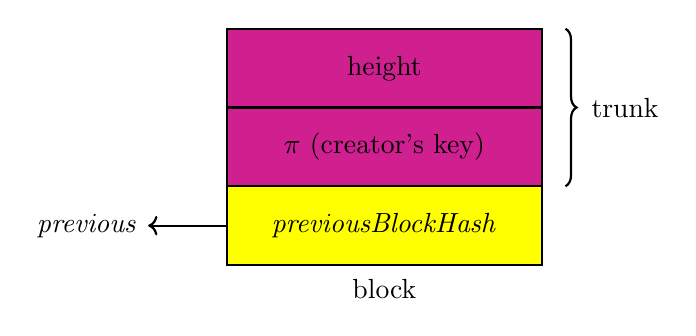
\begin{tikzpicture}
      \draw [decorate,decoration={brace,amplitude=4pt},thick,xshift=0.3cm,yshift=0pt]
      (4,7.5) -- (4,5.5) node [midway,right,xshift=.2cm] {trunk};
      \draw [fill=VioletRed, thick] (0,5.5) rectangle (4,7.5);
      \draw (2,7) node{height};
      \draw [fill=VioletRed, thick] (0,4.5) rectangle (4,6.5);
      \draw (2,6) node{$\pi$ (creator's key)};
      \draw [fill=Yellow, thick] (0,4.5) rectangle (4,5.5);
      \draw (2,5) node{$\previousblockhash$};
      \draw[->,thick] (0,5) -- (-1,5) node [midway,left,xshift=-.5cm] {$\previous$};
      \draw (2,4.2) node{block};
    \end{tikzpicture}
  \end{center}
  }

  \visible<3->{
  \begin{center}
    \textbf{Proposition.} Challenges depends on the trunks only (simple proof by induction): Signum has no block-grinding attacks
  \end{center}
  }

\end{frame}

\begin{frame}{Point~3: The delay of a nonce \wrt a challenge}

  \begin{center}
  Let $\challenge={\color{blue}\langle i,\sigma\rangle}$ and
  $\nonce=\langle p,\underbrace{h_0,h_{2n-1}}_{\scoop_0},\underbrace{h_2,h_{2n-3}}_{\scoop_1},\ldots,\underbrace{h_{2n-4},h_3}_{\scoop_{n-2}},\underbrace{h_{2n-2},h_1}_{\scoop_{n-1}}\rangle$:
  \end{center}
  \bigskip
  \[
    \delay(\nonce,\challenge)=\hash(\scoop_{\color{blue}i}\bowtie{\color{blue}\sigma})
  \]

\end{frame}

\begin{frame}[fragile]{Signum's proof of space mining}
 
\begin{algorithm}[H] 
\caption{Signum's Proof of Space}
\begin{algorithmic}[1]
\Require{$block$, non-empty $plot$ file created by $\pi$}
\Ensure{$next$ (a valid child of $block$)}
\Statex
\State {$best\_nonce$ $\gets$ first nonce of $plot$}
\State {$c$ $\gets$ $\challenge(block)$}
\For{$nonce \in plot$}
\If{$\delay(nonce, c)$ $<$ $\delay(best\_nonce, c)$}
\State {$best\_nonce$ $\gets$ $nonce$}
\EndIf
\EndFor
\State \Return {valid block pointing back to $block$, created by $\pi$ and using $best\_nonce$}
\end{algorithmic}
\end{algorithm} 

\end{frame}

\begin{frame}{Miner $\pi$ selects its $\bestNonce$ and builds a next block}

  \begin{center}
    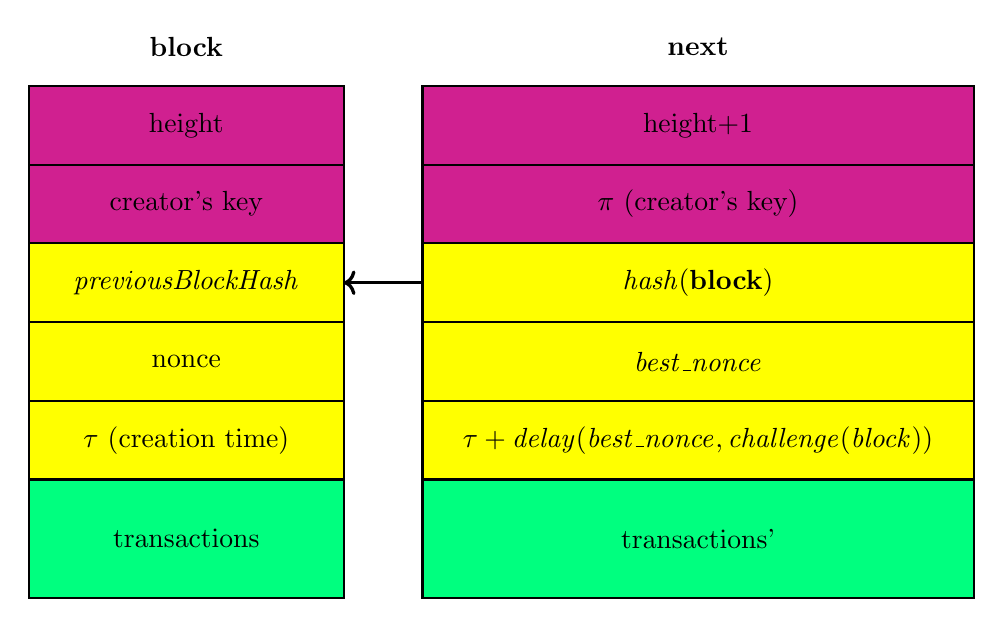
\begin{tikzpicture}
      \draw (2,7) node{\textbf{block}};
      \draw [fill=VioletRed, thick] (0,4.5) rectangle (4,6.5);
      \draw (2,6) node{height};
      \draw [fill=VioletRed, thick] (0,3.5) rectangle (4,5.5);
      \draw (2,5) node{creator's key};
      \draw [fill=Yellow, thick] (0,3.5) rectangle (4,4.5);
      \draw (2,4) node{$\previousblockhash$};

      \draw [fill=Yellow, thick] (0,2.5) rectangle (4,3.5);
      \draw (2,3) node{nonce};
      \draw [fill=Yellow, thick] (0,1.5) rectangle (4,2.5);
      \draw (2,2) node{$\tau$ (creation time)};

      \draw [fill=SpringGreen, thick] (0,0) rectangle (4,1.5);
      \draw (2,0.75) node{transactions};

      \visible<2->{
      \draw (8.5,7) node{\textbf{next}};
      \draw [fill=VioletRed, thick] (5,5.5) rectangle (12,6.5);
      \draw (8.5,6) node{height+1};
      }
      \visible<3->{
      \draw [fill=VioletRed, thick] (5,4.5) rectangle (12,5.5);
      \draw (8.5,5) node{$\pi$ (creator's key)};
      }
      \visible<4->{
      \draw [fill=Yellow, thick] (5,3.5) rectangle (12,4.5);
      \draw (8.5,4) node{$\hash(\mathbf{block})$};
      \draw[->,very thick] (5,4) -- (4,4);
      }

      \visible<5->{
      \draw [fill=Yellow, thick] (5,2.5) rectangle (12,3.5);
      \draw (8.5,3) node{$\bestNonce$};
      }
      \visible<6->{
      \draw [fill=Yellow, thick] (5,1.5) rectangle (12,2.5);
      \draw (8.5,2) node{$\tau+\delay(\bestNonce,\challenge(\block))$};
      }

      \visible<7->{
      \draw [fill=SpringGreen, thick] (5,0) rectangle (12,1.5);
      \draw (8.5,0.75) node{transactions'};
      }
    \end{tikzpicture}
  \end{center}

\end{frame}

\begin{frame}{Mokamint}

  \begin{center}
    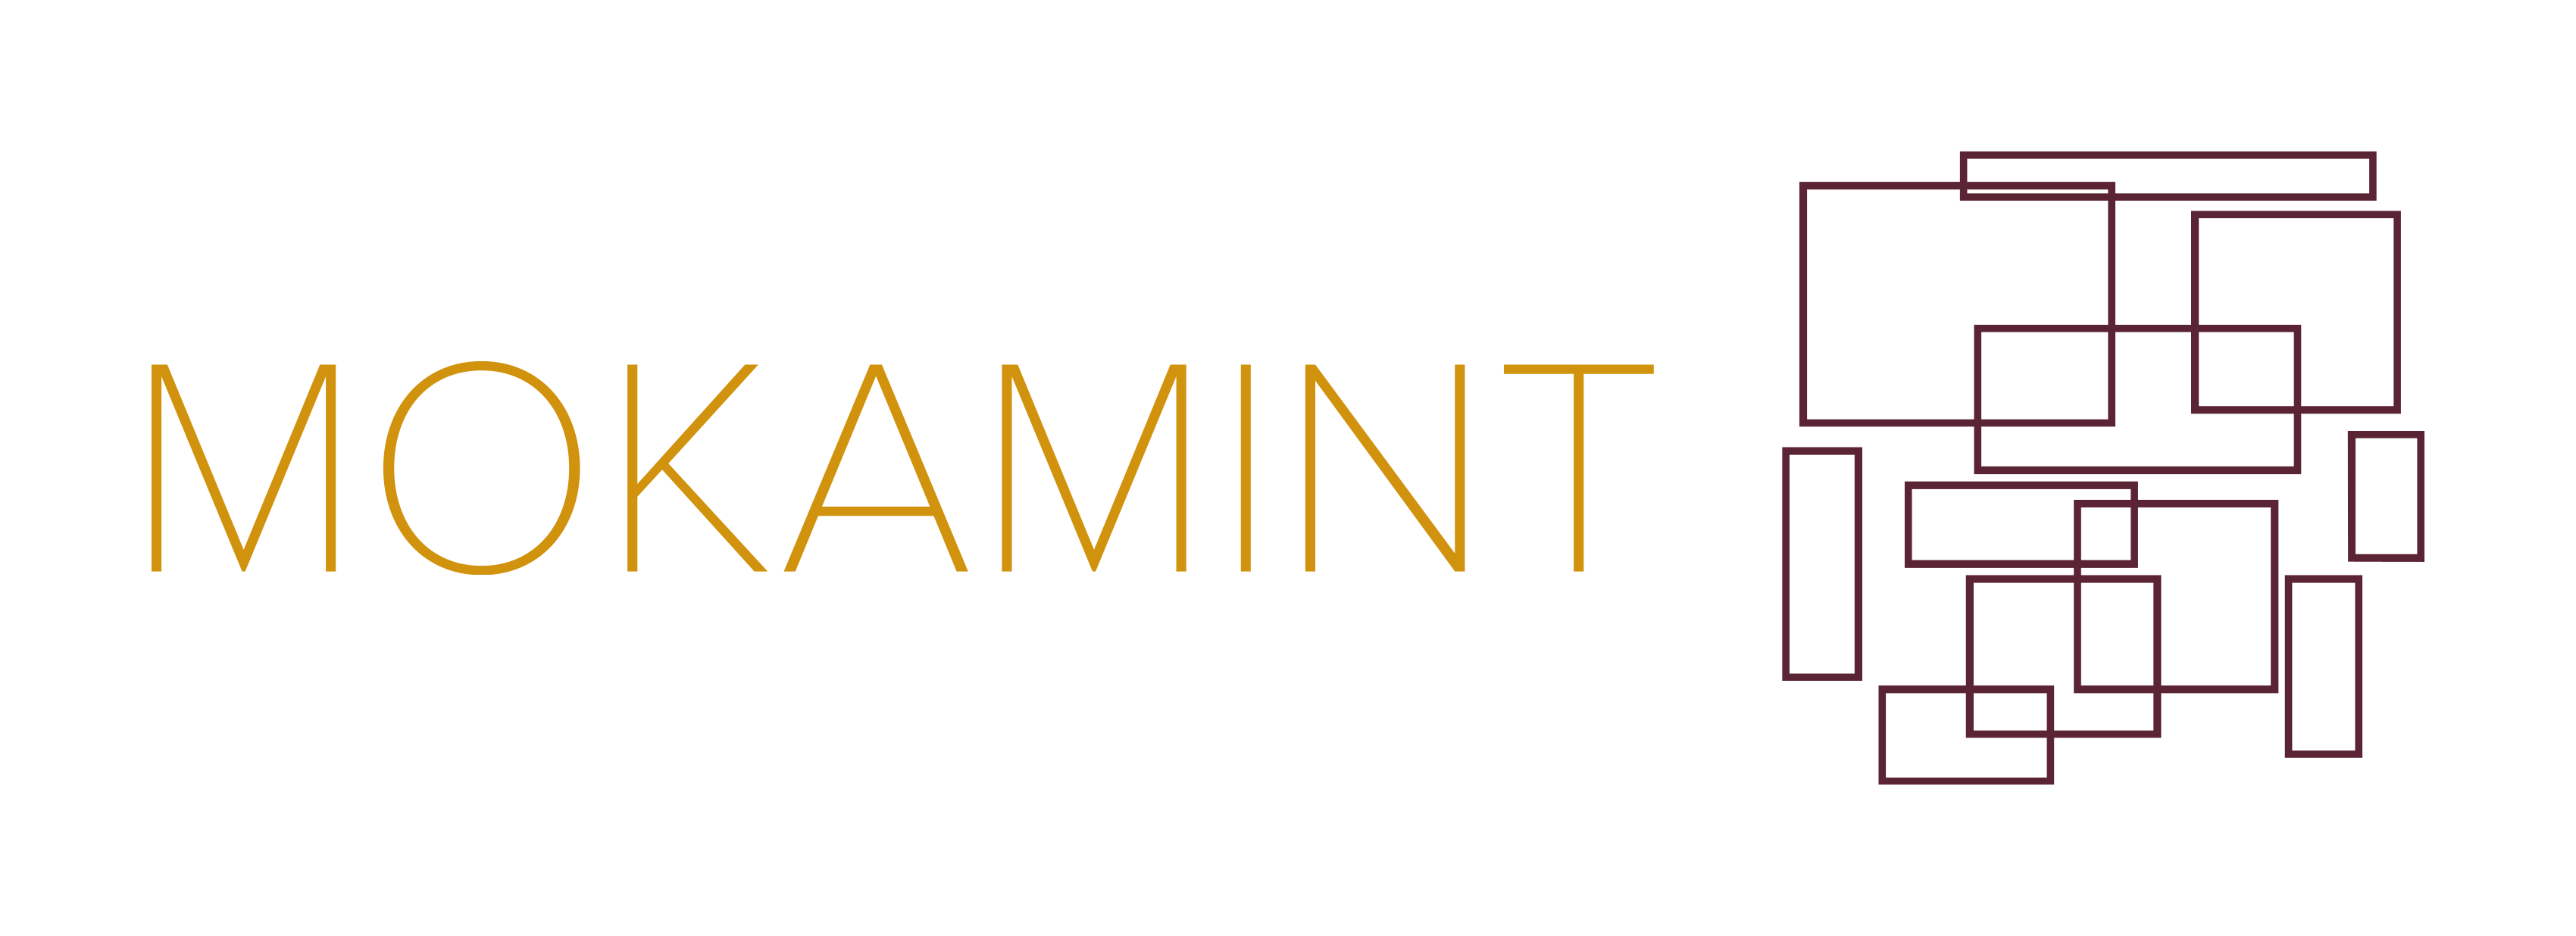
\includegraphics[width=0.4\textwidth]{pictures/mokamint_logo}\\
    \url{https://github.com/Mokamint-chain/mokamint}
  \end{center}


  \begin{center}
    A new blockchain based on proof of space, similar to Signum but \alert{generic}
    wrt.\ the supported \alert{application}
  \end{center}

  \medskip

  \begin{center}
    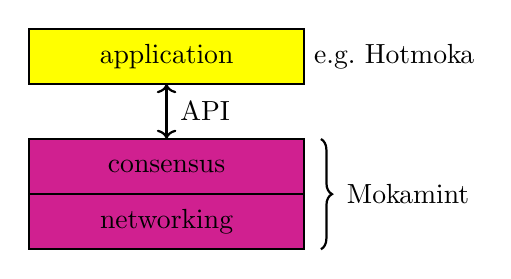
\begin{tikzpicture}[scale=0.7]
      \draw [fill=VioletRed, thick] (0,0) rectangle +(5,1);
      \draw (2.5,0.5) node{networking};
      \draw [fill=VioletRed, thick] (0,1) rectangle +(5,1);
      \draw (2.5,1.5) node{consensus};
      \draw[<->, thick] (2.5,2) -- (2.5,3);
      \draw (3.2,2.5) node{API};
      \draw [fill=Yellow, thick] (0,3) rectangle +(5,1);
      \draw (2.5,3.5) node{application};
      \draw (5,3.5) node [right] {e.g.\ Hotmoka};
      \draw [decorate,decoration={brace,amplitude=4pt},thick,xshift=0.3cm,yshift=0pt]
      (5,2) -- (5,0) node [midway,right,xshift=.2cm] {Mokamint};
    \end{tikzpicture}
  \end{center}

\end{frame}

\begin{frame}[fragile]{Become a miner of the Mokamint+Hotmoka testnet}

  \begin{greenbox}{Mine with the previoulsy created plot file}
\begin{verbatim}
docker run -it \
 -e MINER_PUBLIC_SERVICE_URI=ws://panarea.hotmoka.io:8025 \
 -v miner_configuration:/home/mokamint/miner_configuration \
 mokamint/mokamint:1.3.1 mine
\end{verbatim}
  \end{greenbox}

\end{frame}

\begin{frame}[fragile]{Check that your miner contributes to the blockchain}

  \begin{greenbox}{Show the topmost $20$ blocks of the blockchain}
\begin{verbatim}
docker run --rm -it mokamint/mokamint:1.3.1 \
 mokamint-node chain ls 20 \
 --uri ws://panarea.hotmoka.io:8030
\end{verbatim}
  \end{greenbox}

\end{frame}

\begin{frame}\frametitle{Conclusion}

  The only existing formalization of Signum

  \begin{itemize}
  \item it clarifies how Signum works
  \item it proves that a suspected time-memory trade-off does not exist (but others might exist! a general proof is still missing)
  \item it proves that block-grinding attacks cannot occur
  \item it proves that challenge-grinding attacks are impractical
  \item it proves that Signum is immune from censorship attacks
  \item it introduces a new protection against newborn attacks
  \item it supports the clean, generic Mokamint implementation
  \end{itemize}

\end{frame}

\end{document}
